%%%%%%%%%%%%%%%%%%%%%%% file template.tex %%%%%%%%%%%%%%%%%%%%%%%%%
%
% This is a general template file for the LaTeX package SVJour3
% for Springer journals.          Springer Heidelberg 2010/09/16
%
% Copy it to a new file with a new name and use it as the basis
% for your article. Delete % signs as needed.
%
% This template includes a few options for different layouts and
% content for various journals. Please consult a previous issue of
% your journal as needed.
%
%%%%%%%%%%%%%%%%%%%%%%%%%%%%%%%%%%%%%%%%%%%%%%%%%%%%%%%%%%%%%%%%%%%
%
% First comes an example EPS file -- just ignore it and
% proceed on the \documentclass line
% your LaTeX will extract the file if required
%\begin{filecontents*}{example.eps}
%!PS-Adobe-3.0 EPSF-3.0;
%%BoundingBox: 19 19 221 221
%%CreationDate: Mon Sep 29 1997
%%Creator: programmed by hand (JK)
%%EndComments
%gsave
%newpath
%  20 20 moveto
%  20 220 lineto
%  220 220 lineto
%  220 20 lineto
%closepath
%2 setlinewidth
%gsave
%  .4 setgray fill
%grestore
%stroke
%%grestore
%\end{filecontents*}
%
%\RequirePackage{fix-cm}
%
%\documentclass[twocolumn,a4paper]{svjour3}                     % onecolumn (standard format)
%\documentclass[smallcondensed]{svjour3}     % onecolumn (ditto)
%\documentclass[smallextended]{svjour3}       % onecolumn (second format)
%\documentclass[twocolumn]{svjour3}          % twocolumn
%
%\smartqed  % flush right qed marks, e.g. at end of proof
%
% -------------------------------------------- %
%\documentclass[a4paper, 12 pt]{article}  % Comment this line out if you need a4paper
%
%\usepackage{graphicx}
%\usepackage{longtable,lscape}
%\usepackage{gensymb}
%\usepackage{multirow}
%\usepackage{epstopdf} % by Kong
%\usepackage{subfigure} % by Kong
%\usepackage{amsmath} 
%\usepackage{url}
% 
%\usepackage{color}
%\usepackage{latexsym,setspace,amssymb,amsmath,multirow,graphicx,algorithm,algorithmic,subfigure,geometry}
%\linespread{1}
%\geometry{left=1.9cm,right=1.9cm,top=2.54cm,bottom=1.9cm}
% -------------------------------------------- %

\documentclass[letterpaper,12pt]{article}
\renewcommand{\baselinestretch}{1.5}
\renewcommand*\footnoterule{}
\usepackage{times}
\usepackage[margin=1in]{geometry}
\newcommand*\apostrophe{\textsc{\char39}}
\setlength{\paperheight}{11in}
\setlength{\paperwidth}{8.5in}
\usepackage{graphicx}
\DeclareGraphicsExtensions{.pdf,.jpeg,.png}
\usepackage{cite}
\usepackage{amsmath}
\usepackage{titlesec}

\usepackage{graphicx}
\usepackage{longtable,lscape}
\usepackage{gensymb}
\usepackage{multirow}
\usepackage{epstopdf} % by Kong
\usepackage{subfigure} % by Kong
\usepackage{amsmath} 
\usepackage{url}


\titlelabel{\thetitle.\quad}
\titleformat*{\section}{\normalfont\bfseries}
\titleformat*{\subsection}{\normalfont\bfseries}
\titleformat*{\subsubsection}{\normalfont\bfseries}
\titleformat*{\paragraph}{\normalfont\bfseries}
\titleformat*{\subparagraph}{\normalfont\bfseries}



%\usepackage[style=authoryear]{biblatex}
%\addbibresource{template.bib} % note the .bib is required
%\renewcommand*{\nameyeardelim}{\addcomma\space}

\begin{document}
\date{}
\title{Ground Stereo-Vision-in-Loop Guidance for Safe Landing of Fixed-wing UAVs: Architecture \& Algorithms}
%\subtitle{Do you have a subtitle?\\ If so, write it here}

%\titlerunning{Short form of title}        % if too long for running head

\author{Weiwei Kong, Tianjiang Hu, Daibing Zhang, Lincheng Shen, Jianwei Zhang %etc.
}

%\authorrunning{Short form of author list} % if too long for running head

%\institute{W. Kong \at
%            first address \\
%              Tel.: +123-45-678910\\
 %            Fax: +123-45-678910\\
 %            \email{kongww.nudt@gmail.com}           %  \\
%             \emph{Present address:} of F. Author  %  if needed
%           \and
%           S. Author \at
 %             second address
%}

%\date{Received: date / Accepted: date}
% The correct dates will be entered by the editor


\maketitle

\begin{abstract}
Orchestrating a safe landing is one of the greatest challenges for aircraft. This paper aims to deal with the problem of automatically landing a Unmanned Aircraft Vehicle (UAV) in the field with the help of a ground-based stereo visual system. This novel visual system consists of two separate perception modules which equipped with a pan/tilt unit (PTU) and optical sensors. Benefiting from the large baseline and extended field of view (FOV), our system could locate the aircraft precisely by triangular geometry during the final landing approaching in GNSS-denied or -impaired environments. To track the target at long distance, the Semi-random-code TLD algorithm (SRC-TLD) and Bounding Box Shrinking (BBS) algorithm were designed to improve the location accuracy. We provide the results from both simulation and practical experiments, showing the performance of the novel system and the overall accuracy during the landing process. In addition, this autonomous landing system caters for all of the different UAV system in operation, such as fixed-wing and rotary wing. 

%These two modules setup at the each side of the runway and benefiting from the large baseline and extended field of view (FOV), the aircraft could be tracked at $1\ km$ in distance. The position of the UAV could be calculated by triangular geometry. We provide the results from both simulation and practical experiments, showing the performance of the novel system and the overall accuracy during the landing process. Our approach offer increased accuracy in measuring aircraft position in GNSS-denied scenario when compare to human operation. 
 
\textbf{Keywords: UAV; Stereo Vision; Localization}
% \PACS{PACS code1 \and PACS code2 \and more}
% \subclass{MSC code1 \and MSC code2 \and more}
\end{abstract}

\begin{figure*}[!hb]
	\centering
	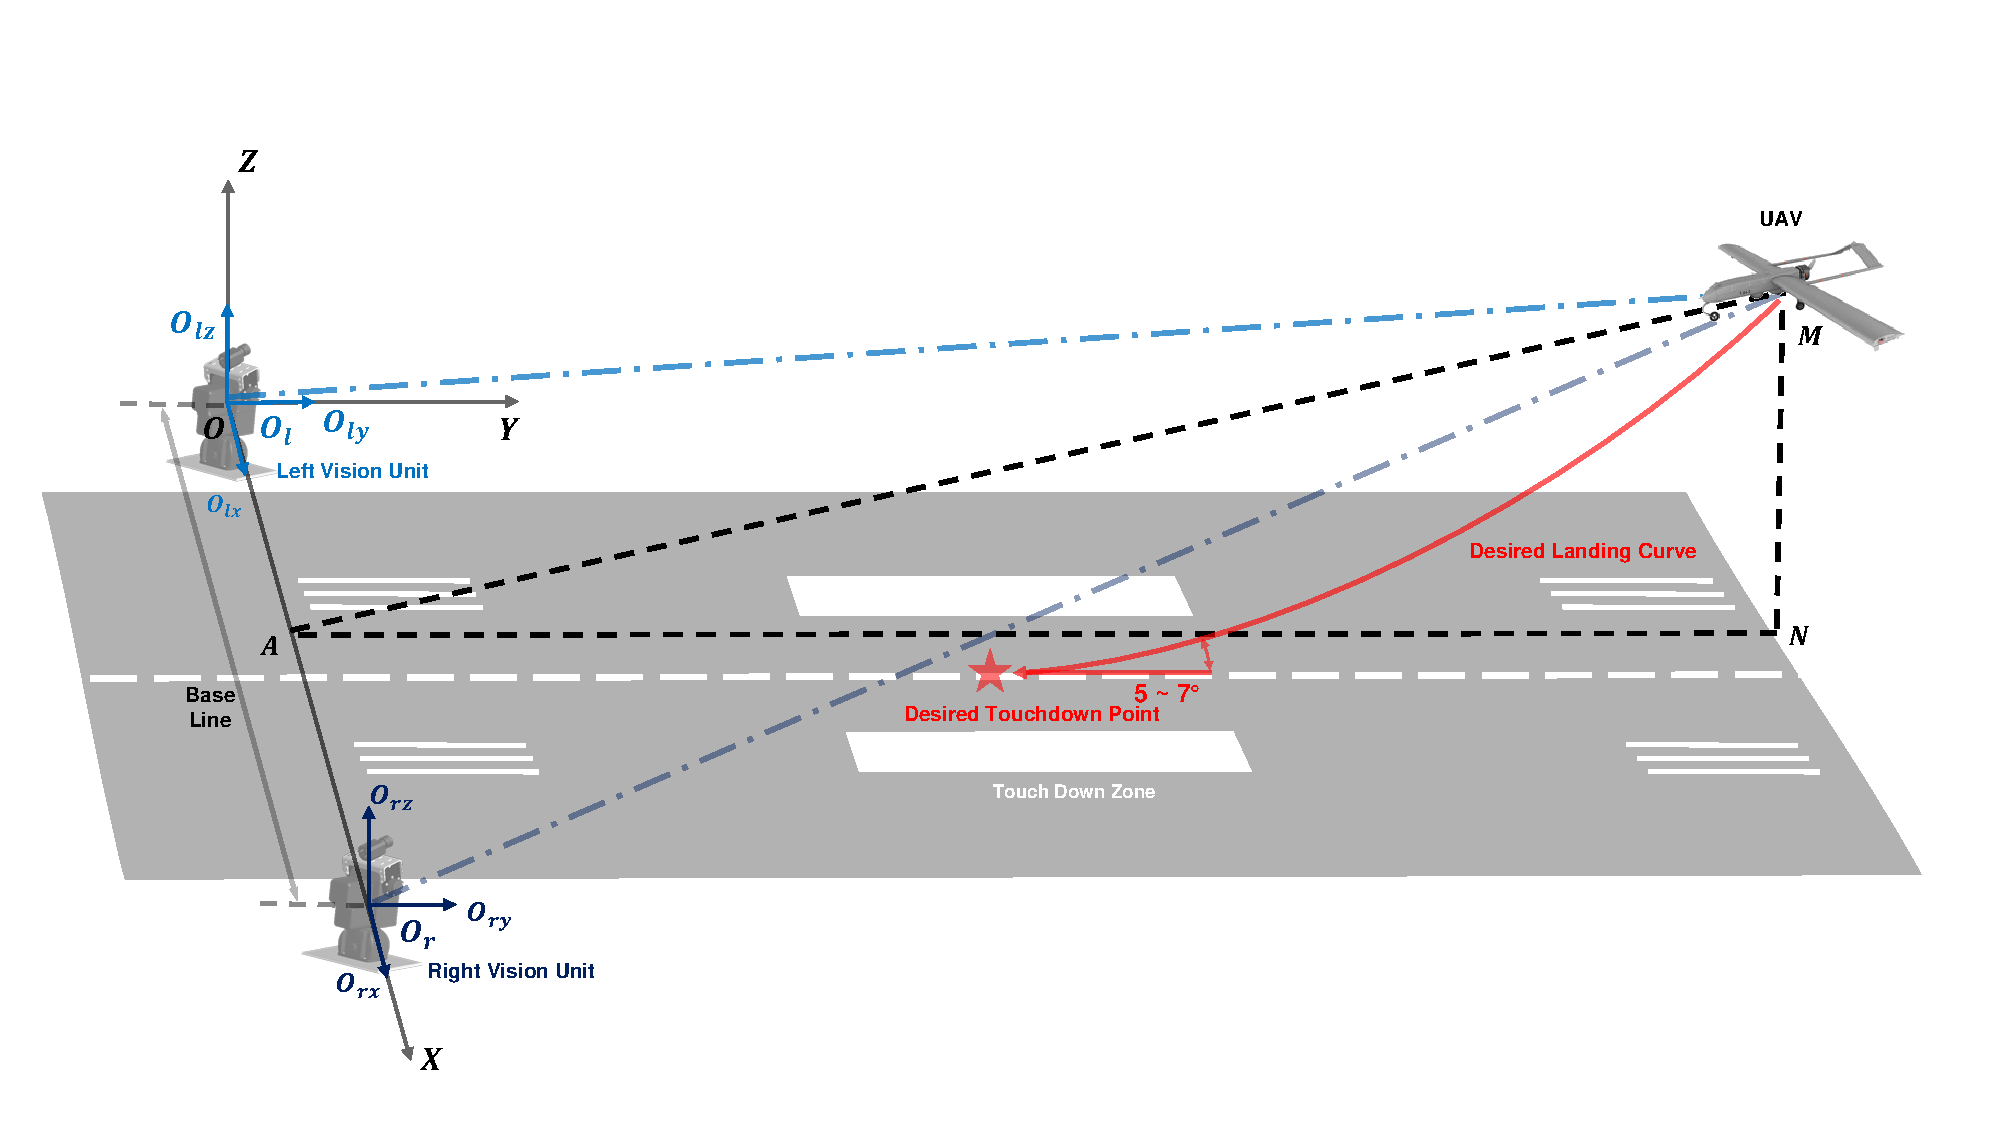
\includegraphics[width=\textwidth]{Figs/Fig04_GeneralSystem.pdf}
	\caption{The separated stereo visual gudiance system.}
	\label{fig:Fig04_GeneralSystem}
\end{figure*}




\section{Introduction}
\label{intro}
%无人机大量应用
In the past decades, the use of unmanned aerial vehicles (UAVs) has increased tremendously in both military and civil fields. Although aerial robots have successfully implemented in several applications, there are still new research directions relate to them. Kumar et al. \cite{kumar2012opportunities} summarized the opportunities and challenges of this growing field, from the model design to high-level perception capability. All of these issues are concentrating on improving the degree of autonomy, which supports UAVs continue to be used in novel and surprising ways.

% 自主降落能力至关重要
No matter fixed-wing platform or rotors aircraft, a standard fully unmanned autonomous system(UAS) involves performing takeoffs, waypoint navigation and landings. Among them, automatic landing is the most delicate and critical phase of a UAV flight. Two technical reports \cite{williams2004summary,manning2004role}, claimed that nearly 50\% of fixed-wing UAVs such as Hunter and Pioneer operated by the US military suffer accidents during landing. Also, almost 70\% of mishaps for Pioneer UAVs occurred during landing due to human factors. So a proper assist system is needed to enhance the reliability of landing task. Generally, two main capabilities of the system are required. The first one is navigation and localization of UAVs, and the second one is generating the appropriate guidance command to guide UAVs for a safe landing. In this paper, we mainly focus on the first issue and try to improve the guidance accuracy and robustness.


% GNSS不行
For manned aircraft, the traditional landing system uses a radio beam directed upward from the ground \cite{mclean1990automatic, stevens2003aircraft}. By measuring the angular deviation from the beam through onboard equipment, the pilot knows the perpendicular displacement of the aircraft in the vertical channel. For the azimuth information, additional equipment is required. However, due to the size, weight, and power (SWaP) constraints, it is impossible to equip these instruments in UAV. Thanks to the GNSS technology, we have seen lots of successful practical applications of autonomous UAVs in outdoor environments such as transportation, aerial photography and intelligent farming. Unfortunately, in some circumstances, such as urban or low altitude operations, the GNSS receiver antenna is prone to lose line-of-sight with satellites and making GNSS unable to deliver high quality position information \cite{farrell1998gps}. So the autonomous landing in unknown or Global Navigation Satellite System(GNSS)-denied environment is still an open problem. 

Visual based approach is an obvious way to achieve the autonomous landing by estimating flight speed and distance to the landing area, in a moment-to-moment fashion. Generally, two types of visual methods can be considered. The first type is the vision-based onboard system, which has been widely studied. The other is to guidance the aircraft using the ground-based camera system. Once the aircraft is detected by the camera during the landing process, its characteristics, such as type, location, heading and velocity, can be derived by the guidance system. Based on these information, the UAV could align itself carefully towards the landing area and adapt its velocity and acceleration to achieve safely landing. In summary, two key elements of the landing problem are detecting the UAV and its motion calculating the location of the UAV relative to the landing filed. 

Motivated by these pressing problems, we introduce a novel ground-based visual landing system. Unless the existing ground-based guidance system that has limited baseline, our proposed approach sets up the camera on a pan-tilt unit (PTU) to increase the effective field of view (FOV) of cameras and the distance at which a reliable lock could be established and maintained. The general view of the fresh guidance system is shown in Figure \ref{fig:Fig04_GeneralSystem}. The key contributions of this papers is threefold:
\begin{itemize}
	\item First, we introduce a novel ground-based guidance system with large baseline and 360° circular coverage, eliminating the dependency of GNSS.
	\item Second, we designed real-time SRC-TLD and BBS tracking and localization framework to guide the aircraft landing safely. 
	\item Third, the whole system has been tested using a fixed-wing aircraft with an appropriate landing strategy.
\end{itemize}



\section{Related Works}

%\subsection{Instrument Approach}
%To achieve better performance in GNSS-denied environment, some military-grade on-ground systems, such as OPATS\cite{RUAG}, DT-ATLS\cite{SierraNevadaCorporation} and UCARS \cite{SierraNevadaCorporationa}, were developed, mainly based on millimeter wave track radar, laser pointer, cooled infrared camera, etc. Yet no further information about these products is publicly available. These systems are shown in Figure.\ref{fig:OPATS}, Figure.\ref{fig:DT_ALTS} and Figure.\ref{fig:UCARS_V2}.
%
%\begin{figure}[!tb]
%	\centering
%	\subfigure[]
%	{
%		\label{fig:OPATS}
%		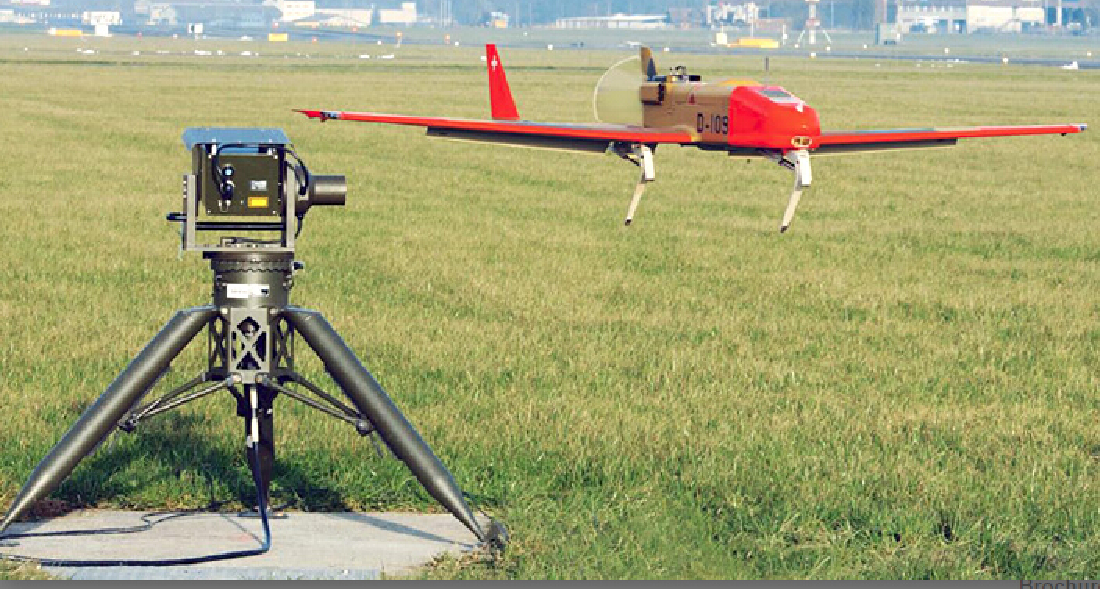
\includegraphics[height=3.5cm]{Figs/07_OPATS.pdf}
%	}
%	\subfigure[]
%	{
%		\label{fig:DT_ALTS}
%		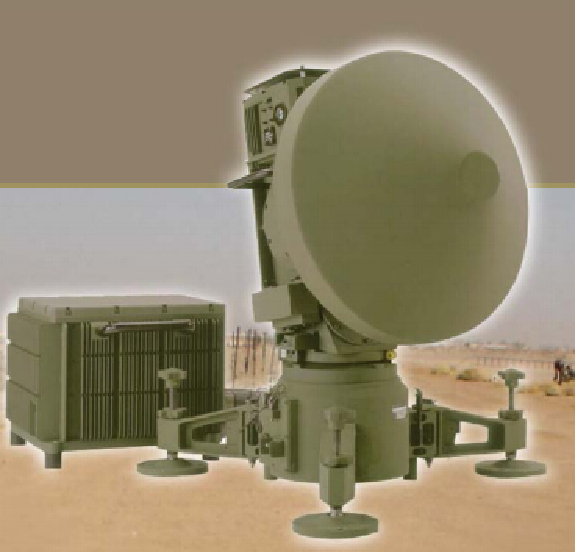
\includegraphics[height=3.5cm]{Figs/08_DT_ALTS.pdf}
%	}
%	\subfigure[]
%	{
%		\label{fig:UCARS_V2}
%		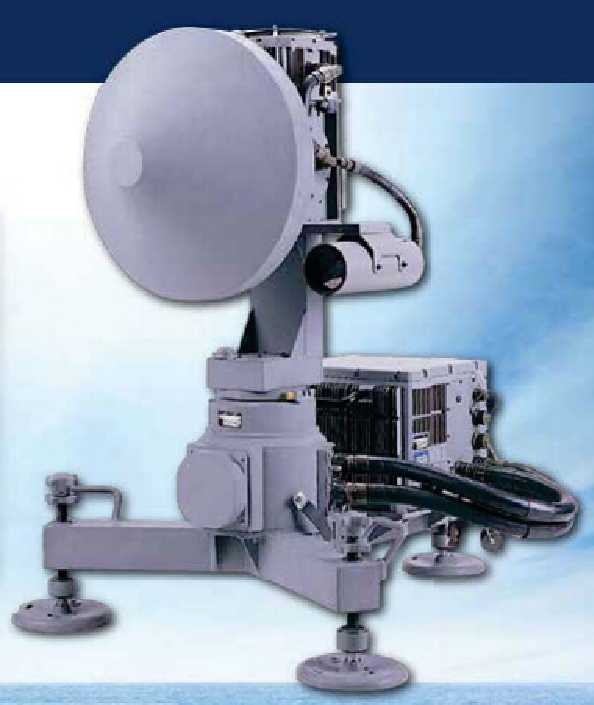
\includegraphics[height=3.5cm]{Figs/09_UCARS_V2.pdf}
%	}	
%	\caption{(a) OPATS (b) DT-ALTS (c) UCARS-V2}
%\end{figure}
%
%The Instrument Landing System (ILS) is widely used in most of the international airports around the world allowing pilots to establish on the approach and follow the ILS, in autopilot or not, until the decision height is reached. This approach refer to a ground-based instrument system providing accurate guidance to a plane takeing-off from a runway or approaching and landing on a runway. A reference book \cite{Nolan2010} provided in-depth discussion of the ILS.

\subsection{On-board Vision Method}
The problem of accurately landing a UAV using vision-based control has been well developed for autonomous rotorcraft. Visual Servo algorithms have been extensively studied in the robotics filed over the past decade. Considering the model as an eye-in-hind configuration, an practical imaged-based visual servo control frame work has been proposed by Guenard \cite{Guenard2008}. By calculating the image error kinematics, a designed Lyapunov controller shows good performance and robustness of hovering a quadrotor UAV. 

%Mej{\'{\i}}as developed an image-based velocity references approach to visually control the altitude and lateral of the helicopter \cite{Mejias2006}. These vision velocity reference is combined with GPS and IMU data for more accurate and position measurements.

An alternative to template-based method are optical-flow-aided position measurement systems. This approach was inspired by flying insect navigation strategies \cite{Green2004} and have been developed over the years to use onboard terrestrial and aerial robots. Triggered by the observations of honeybees, an optic flow regulator was introduced \cite{Ruffier2014}. It allows a tethered rotorcraft to deal with non-stationary environments and the rotorcraft was able to land safely near a target which mounted on a moving platform both vertically and horizontally. In another recent work \cite{Vlantis2015}, a discrete-time non-linear model predictive controller (MPC) was employed to land a Parrot AR.Drone on a Pioneer mobile robot with inclined platform. The on-board forward facing camera was used for tracking the moving target and the downwards pointing camera for optical flow. For fixed-wing aircraft, Kim et al.\cite{Kim2013} reported a vision-based net recovery system. The ground station received the image capture by the on-board camera aiming to detect a recovery net. The longitudinal and lateral bearing angle were calculated in keeping with a guidance law based on the net relative position. This technique is not suitable for the whole landing process because the vision operating range is only 50 m.
 

%  QR-Code
% but no automatic landing was attempted.

For cooperative localization some structured landing mark, such as 2D barcodes, helipad, could provide the relative transform between landing area and camera. Sharp et al. \cite{Sharp2001} solved the landing task of a Yamaha R-50 helicopter by using the designed landing target(white squares) for landing area recognition and estimating the relative position. By calculating the multiple view matrix, their proposed algorithms\cite{Shakernia2002} improve the motion and structure estimation. However, the controller only regulates the x and y position to hover over the landing platform. Saripalli et al. also presented a image-moment-based method for autonomous landing of a helicopter on a H-shape landing pad \cite{Saripalli2003}. However, the precise height estimation benefits from the differential GPS system. In 2012, a worthwhile study \cite{richardsonautomated2013} provide a framework for an automated vision-based recovery of an unmanned rotatory craft onto a moving platform. The onboard camera system calculates the displacement and orientation of the UAV respect to the pattern and autonomous maneuvers the craft towards the landing platform. The workable limit for robust tracking was 10 m. For fixed-wing landing, German Aerospace Center (DLR) built and tested the 44-pound drone which successfully spotted a QR code on the roof of an Audi and touched down on the net affixed to the station wagon’s roof, at 43 mph \cite{DLR_Landing}. However, due to the viewing angle of the lens and the size of fiducial marker, the detection distance of the sole of vision control method is limited.


% TODO 有效探测距离

% Laser  & Visual
The combination of laser and visual system also has a long history in this field. In 2009, Garratt \cite{garrattvisual2009} considered a relatively low-cost guidance system through visual tracking and LIDAR positioning for autonomous recovery of a Yamaha R-max rotorcraft from ships at sea. This onboard visual system identifies and tracks the single beacon to determine both the distance and the orientation of the deck. Because the wavelength of the beacon is 650 nm, the craft can track it in bright sunlight. For the laser system, the laser rangefinder at a wavelength of 780 nm assembling with a spinning mirror was mounted at the bottom of the rotorcraft, which scans a conical pattern on the deck for estimating the position. The error of position estimation is better than 2 cm in practice, but the detection distance is only 100 m due to the size and the power of the selected LED. 

%While there is significant work using electro-optical pod, laser scanner and radar, those methods require more hardware for the aircraft to carry; therefore, in this case, we focus just on ground-based visual case, which is a lighter weight solution for UAV.
% Because laser-based system are in most cases emit radiation and are therefore likely to reveal the aircraft location to hostile forces.
\subsection{Ground-based Vision Method}
While several techniques have been applied for on-board vision-based control of UAVs, few have shown landing of a fixed-wing guiding by ground-based vision system. Wang \cite{Wang2006} proposed a system using a step motor controlling web camera to track and guide a micro-aircraft. The drawback of this system is the limited baseline leading to a narrow field of view (FOV). To increase the camera FOV, multi-camera systems are considered attractive. This kind of system could solve the common vision problems and track object to compute their 3D locations. At Chiba University \cite{pebrianti2010autonomous}, a ground-based Bumblebee stereo vision system was used to calculate the 3D position of a quadrotor at the altitude of 6 meter. 

In addtion, Martinez \cite{Martinez2009a} introduced a trinocular on-ground system, which is composed by three or more cameras for extracting key features of UAV in order to obtain robust 3D position estimation. The range of detection is still not sufficient for fixed-wing UAV. And another drawback of multi-camera system is the calibration process, whose parameters are nontrivial to obtain. Moreover, we also reviewed various vision-based landing approaches performing on different platform \cite{kong2014vision} and Gautam etc. provide another general review of the autonomous landing techniques for UAVs \cite{Gautam2014}.

 

\section{Ground-based Stereo Localization System Architechture}
In this section, we introduce the theoretical model for ground-to-air visual system. We first recap the traditional stereo vision model which has limited base line restrainting the detection distance. To enlarge the system working boundary, we setup the camera and other sensor module on the two separated PTU and then calculate the target according the image information and rotation angle from PTU.

\subsection{Traditional Stereo Vision Model}
The standard camera model is pin-hole camera Mode. The coordinate of the target $M$ is $(x,y,z)$, and its position on image plane is $(u,v)$. The camera focus is $f$, then the relationship of coordinate between the 3D world and 2D image plane can be calculated by 
\begin{equation}
\lambda\left[ {\begin{array}{*{20}{c}}
	u \\ 
	v \\ 
	f 
	\end{array}} \right] =\left[ {\begin{array}{*{20}{c}}
	x \\ 
	y \\ 
	z 
	\end{array}} \right]
\end{equation}
where $\lambda$ is the scale factor. When using eudilar coordinate, we could get
\begin{equation}
\left[ {\begin{array}{*{20}{c}}
	u \\ 
	v 
	\end{array}} \right] =\frac{f}{z} \left[ {\begin{array}{*{20}{c}}
	x \\ 
	y   
	\end{array}} \right]
\end{equation}

%Assuming the camera focus $f$ and the image size $(w_u,w_v)$ is known, the horizontal FOV of camera $\alpha_{FOV}$ can be calculated by
%\begin{equation}
%\tan{\frac{\alpha_{FOV}}{2}}=\frac{w_u}{f}
%\end{equation}
%Similarly, we can prove that the vertical FOV of camera $\beta_{FOV}$ is
%\begin{equation}
%\tan{\frac{\beta_{FOV}}{2}}=\frac{w_v}{f}
%\end{equation}
%When calculating the FOV, the unit of $f$ and $(w_u,w_v)$ should be same, such as pixel or $mm$.

Although the above model is simple, it could be helpful to estimate the theoretical camera lens according the expected distance and resolution or to measure the target size roughly based on the pixel length on image plane. Let the width and height of the target be $W$ and $H$, the distance between the camera and target be $L$, the target projection on image plane be $w$ and $h$, the relationship between them is  
\begin{align}
f=\frac{wL}{W} \\
f=\frac{hL}{H}
\end{align}

When the optical axes of these two cameras are parallel, we could calculate the target in 3D space by
\begin{equation}
\left[ {\begin{array}{*{20}{c}}
	x \\ 
	y \\ 
	z 
	\end{array}} \right] =\frac{b}{d} \left[ {\begin{array}{*{20}{c}}
	u_l \\ 
	u_r \\ 
	f 
	\end{array}} \right]
\end{equation}
where $b$ is the baseline and $d=u_l-u_r$ is the pixel disparity. The traditional stereo vision model as shown in Fig. \ref{fig:chp03_vision_20_basic_stereo}. Even though some calibration methods could manage the axes unparallel situation, it is still difficult to calculate the system correctly as the baseline is large.

\begin{figure}[!tb]
	\centering
	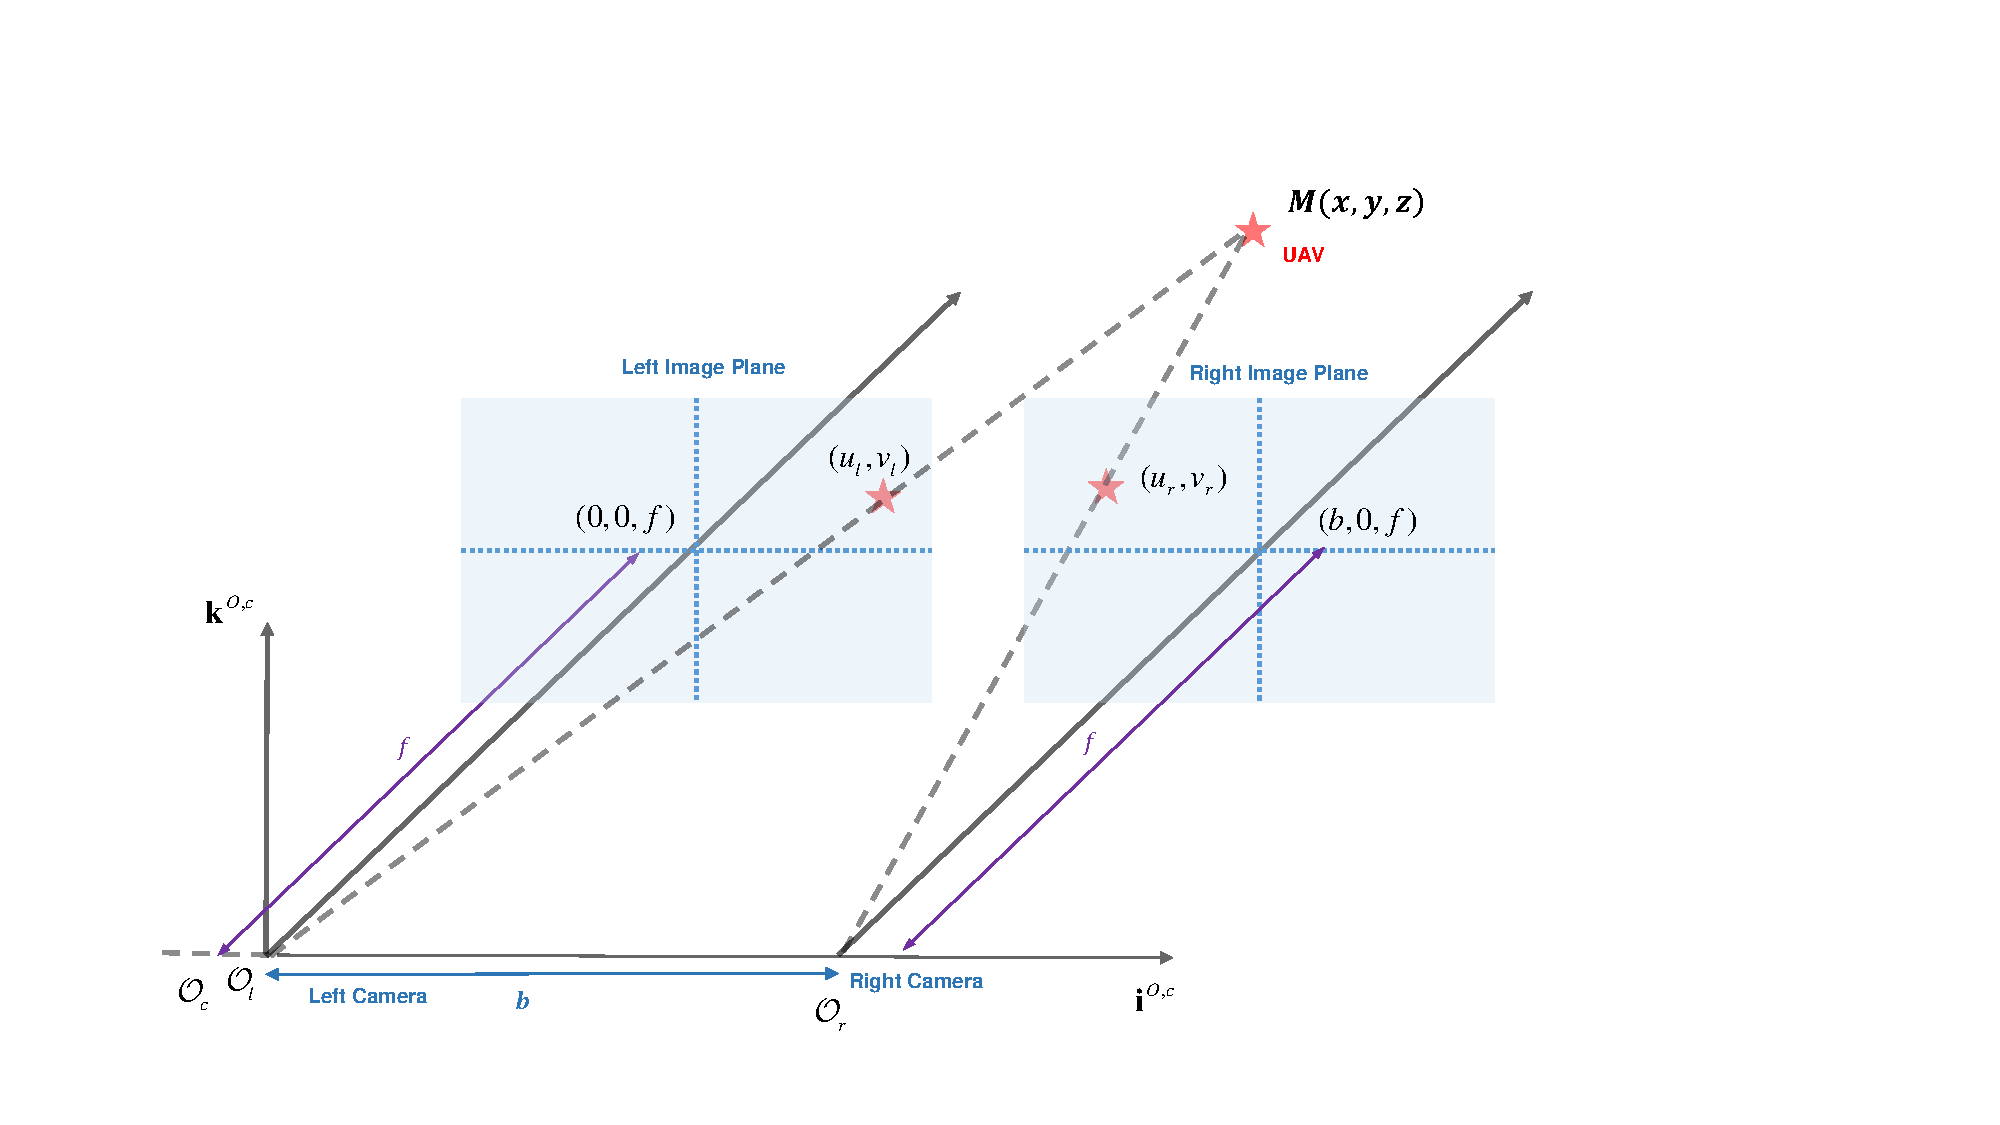
\includegraphics[width=0.6\textwidth]{figs/chp03_vision_20_basic_stereo.pdf}	
	\caption{Theoretical Stereo Vision Model}
	\label{fig:chp03_vision_20_basic_stereo}
\end{figure}

\subsection{Separate Stereo Vision System Configuration}
In order to detect the target at long distance, the large base line, more than $5\ m $, is required. Benefiting the camera assembled on PTU separately, we could switch the baseline freely according to the expected detection distance and target size.

In this paper, we assumed that the world coordinate system $(X, Y, Z)$ is located on the origin of the left vision unit, the rotation center of the PTU. For the sake of simplicity, the camera is installed on the PTU in the way that the axes of the camera frame are parallel to those of PTU frame. The origins of these two frames are close. So it can be assumed that the camera frame coincides with the body frame. Fig. \ref{fig:TheoreticalModel} reveals the theoretical model for visual measurement. After installing the right camera system on ${X}$-axis, the left and right optical center can be expressed as ${O_l}$ and ${O_r}$ respectively. Then the base line of the optical system is $O_lO_r$ whose distance is ${D}$. Considering the center of mass of UAV as a point ${M}$, ${O_lM}$ and ${O_rM}$ illustrate the connections between the each optical center and the UAV. In addition, ${\phi_l}$, ${\phi_r}$, ${\psi_l}$, ${\psi_r}$ denote the tilt and pan angle on both side. Therefore, we define $\phi_l= 0$, $\phi_r=0$, ${\psi_l=0}$ and ${\psi_r=0}$, as the PTU is set to the initial state, i.e. the optical axis parallel the runway; the measurement of a counterclockwise direction is positive.

\begin{figure}[!tb]
	\centering
	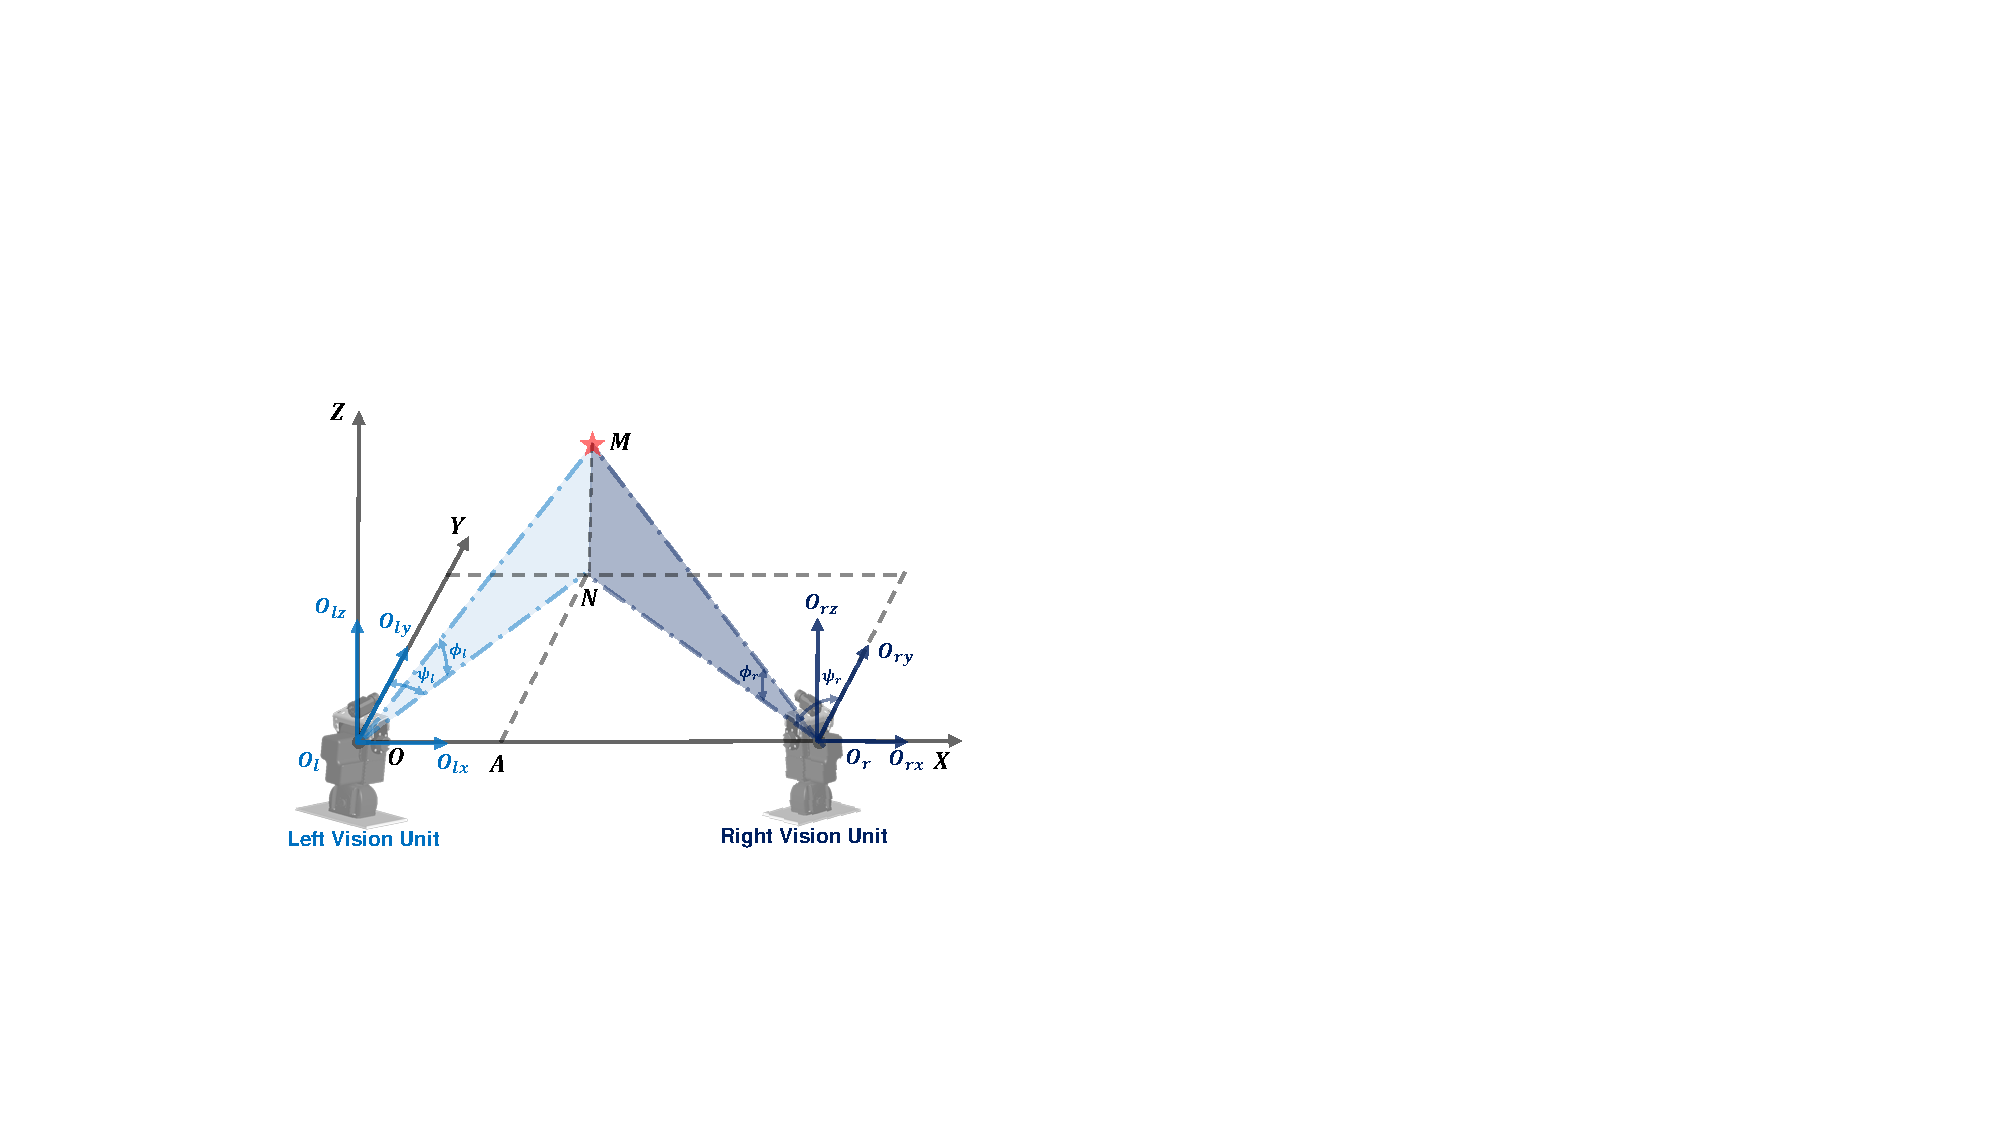
\includegraphics[height=6cm]{figs/Fig03_Stereo.pdf}	
	\caption{Theoretical Optical Model. The target $M$ is projected at the center of the optical axis.}
	\label{fig:TheoreticalModel}
\end{figure}


Since the point ${M}$ not coincides with the principle point which is the center of image plane, the pixel deviation compensation in the longitudinal and horizontal direction should be considered. As shown in Fig. \ref{fig:Fig02_ImagePlaneOnly}, we calculate pixel deviation compensation on the left side by 

\begin{equation} 
\left \{
	\begin{split}
		& \psi_{cl} = \arctan \frac{(u-u_0)du}{f} \\
		& \phi_{cl} = \arctan \frac{(v-v_0)\cos\psi_{cl}dv}{f} 
	\end{split}
\right.
\end{equation}
where optical point is $o(u_o,v_o)$, $du$ and $dv$ are the pixel length of the $u$- and $v$-axis in image plane, and $f$ is the focus. The current PTU rotation angle can be directly obtained through the serial ports during the experiments. Let $\phi_{pl}$ and $\psi_{pl}$ be the left pan and tilt angle separately. Then, the total pan and tilt angle on the left side can be detailed as:
\begin{equation} 
\left \{
	\begin{split}
	    \phi_l &= \phi_{cl} + \phi_{pl} \\ 
	    \psi_l &= \psi_{cr} + \psi_{pr}
	\end{split}
\right.
\end{equation}

\begin{figure*}[!th]
	\centering
	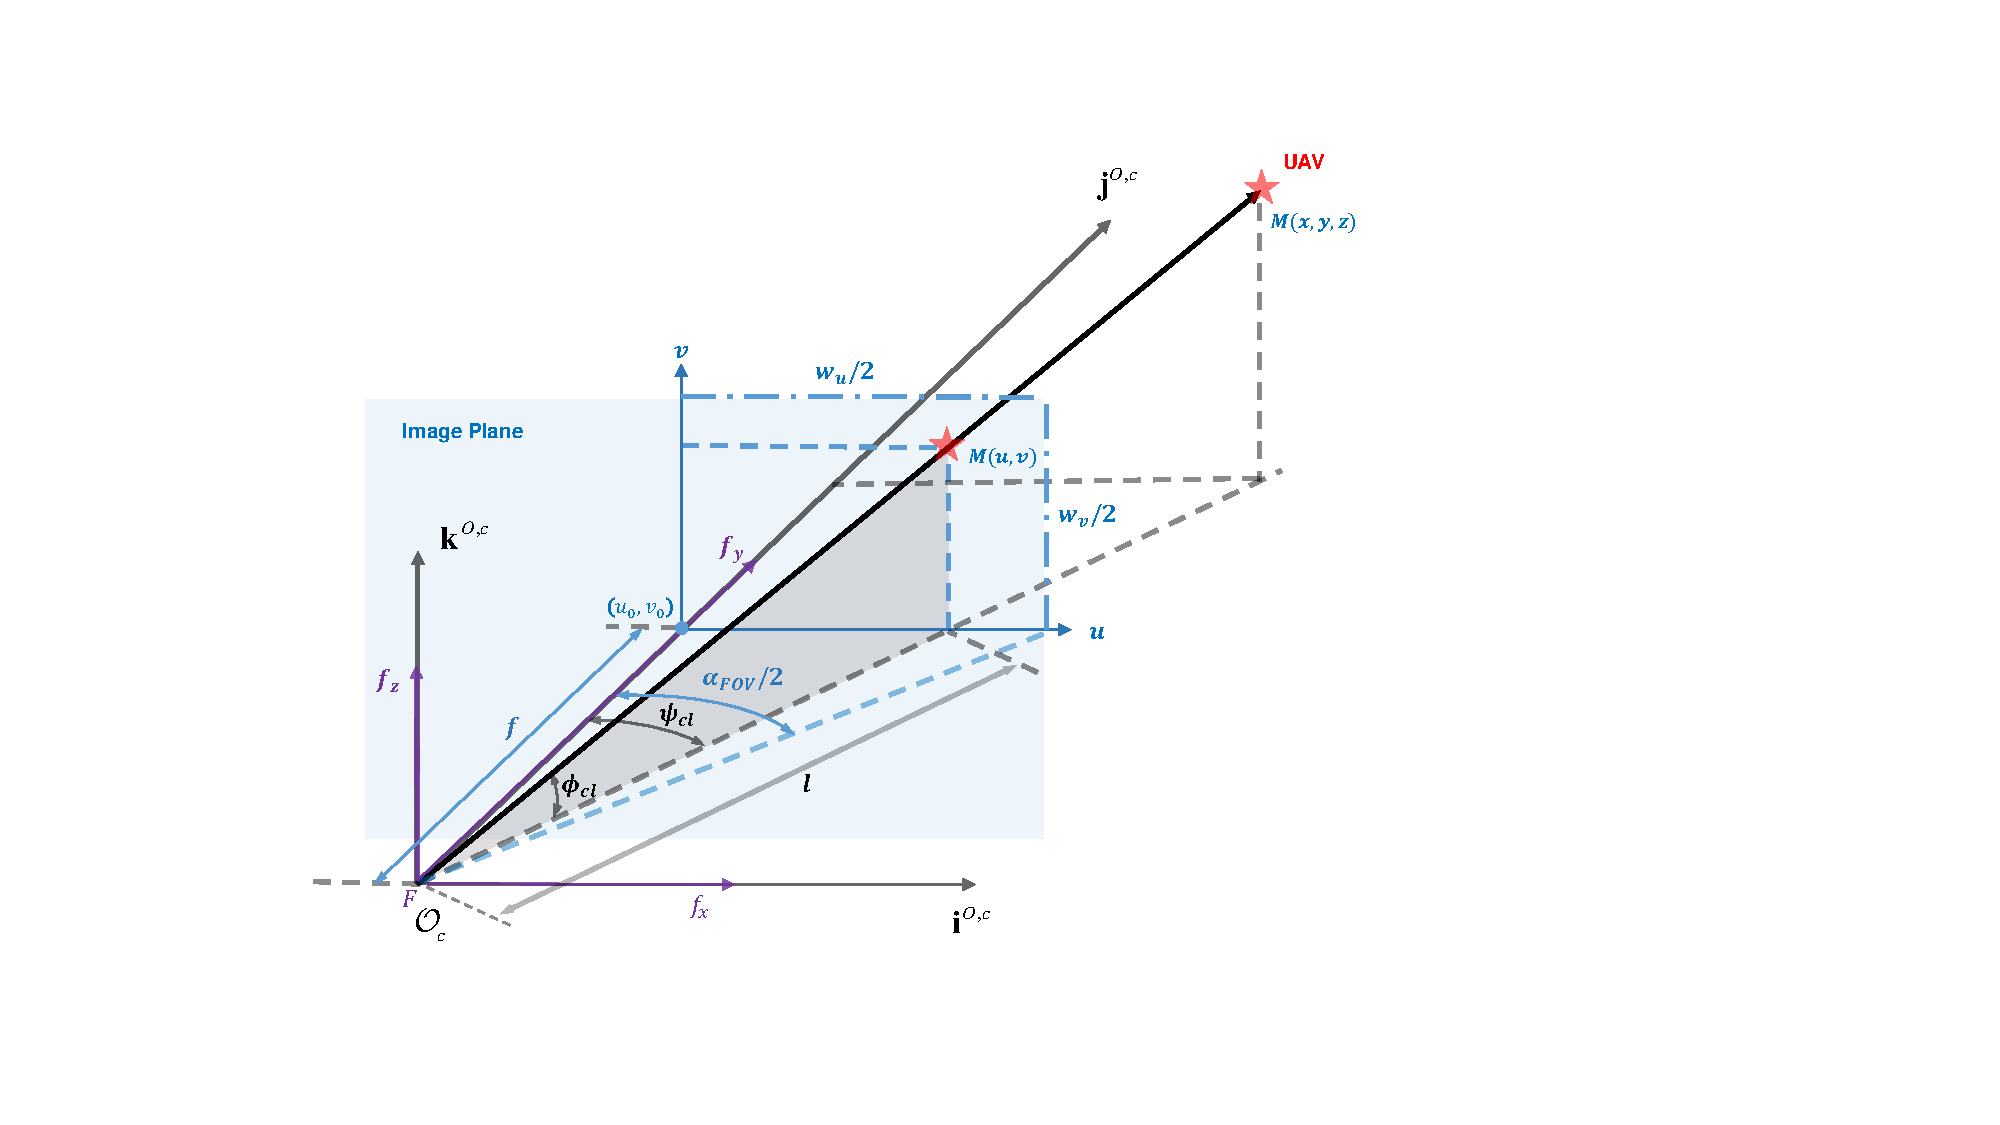
\includegraphics[width=0.6\textwidth]{Figs/chp03_vision_02_image_plane.pdf}
	\caption{The geometry of one PTU with respect to optical center and image plane.}
	\label{fig:Fig02_ImagePlaneOnly}
\end{figure*}

%\begin{figure}[!tb]
%	\centering
%	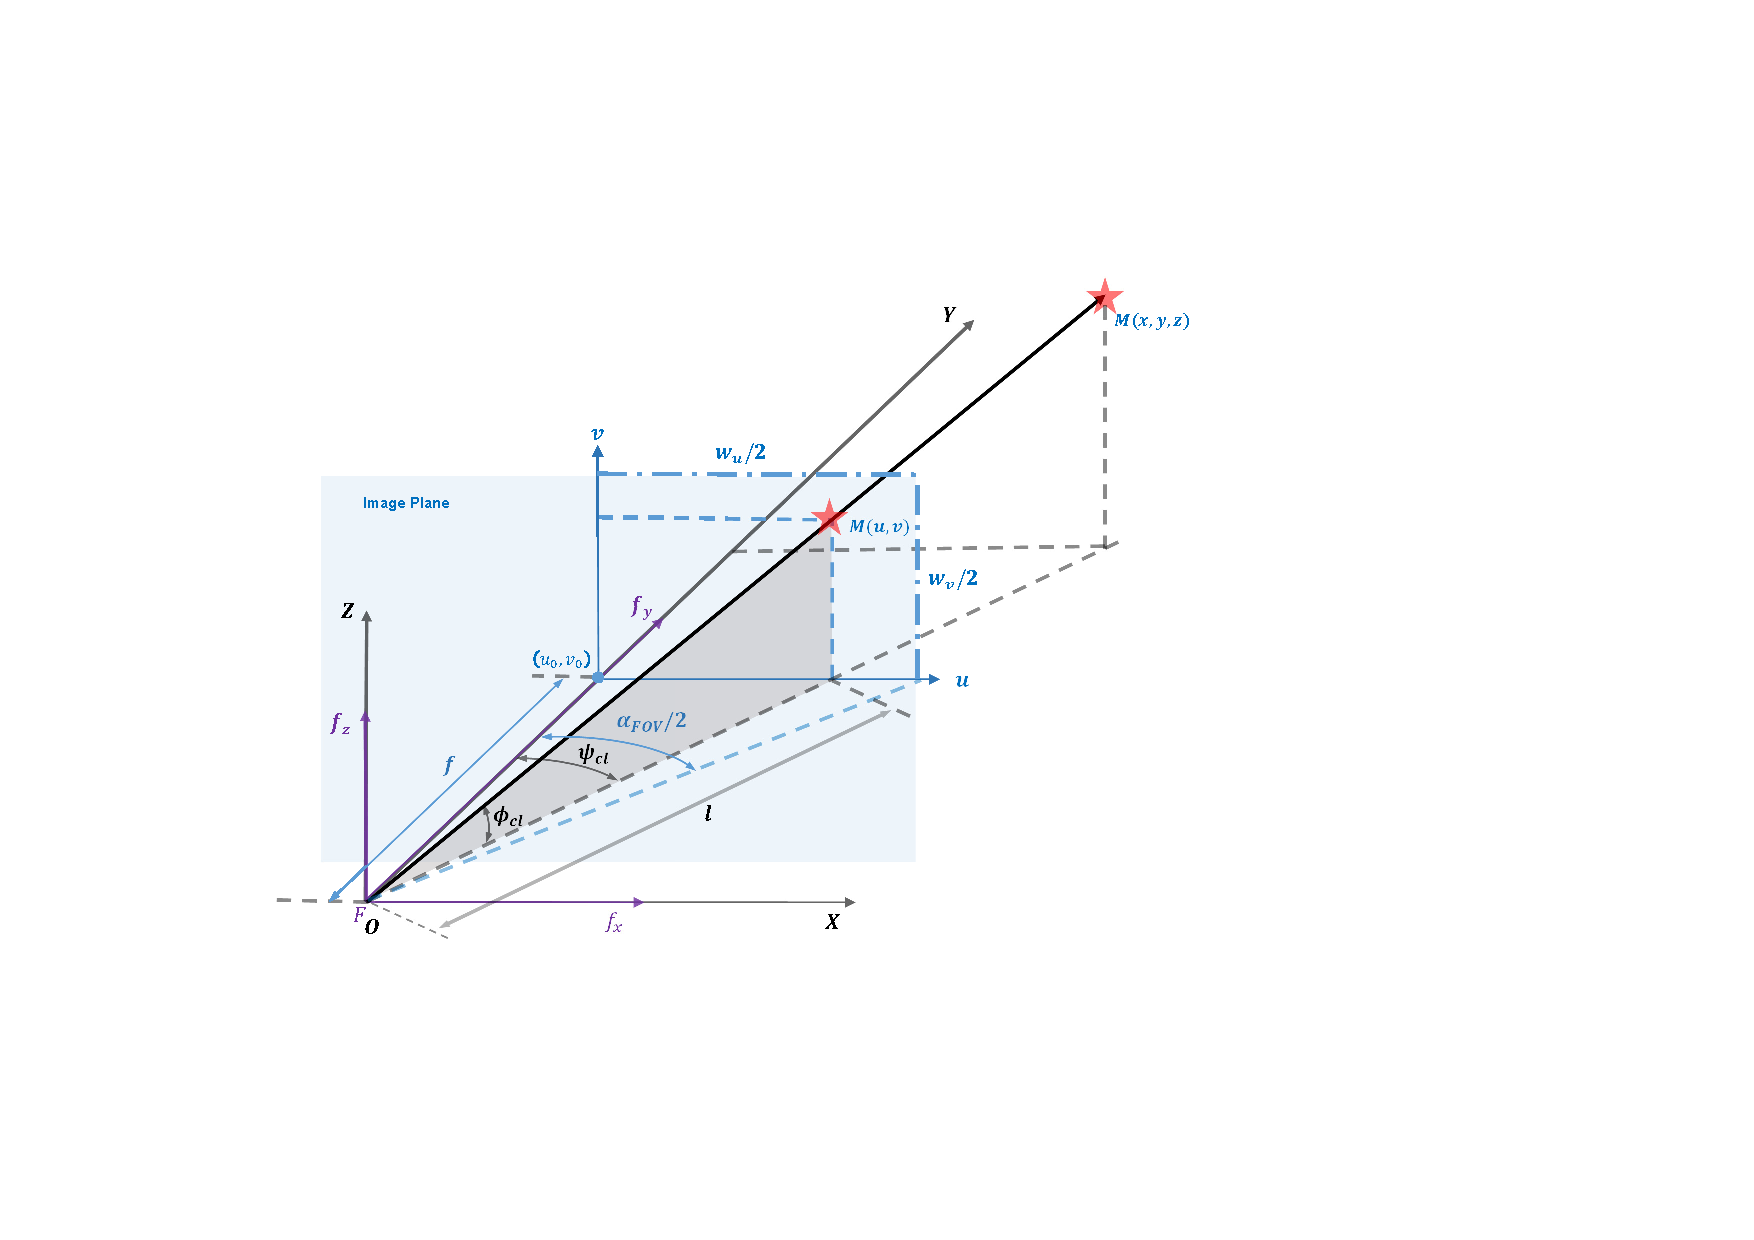
\includegraphics[width=0.5\textwidth]{Figs/Fig02_ImagePlaneOnly.pdf}
%	\caption{The geometry of one PTU with respect to optical center and image plane.}
%	\label{fig:Fig02_ImagePlaneOnly}
%\end{figure}

For the other side, we could also calculate the angle in the same way.

The world coordinates of point ${M}$ is $(x_M, y_M, z_M)\in \textbf{R}^3 $. Point $N$ is the vertical projection of point $M$ on $XOY$ plane, and $NA$ is perpendicular to $X$-axis. If we define $NA = h$, the following guidance parameters can be obtained:
\begin{equation}
\left \{
\begin{aligned}
&x_M = h \tan \psi_l = \frac{D\tan \psi_l}{\tan \psi_l - \tan \psi_r}            \\
&y_M = h = \frac{D}{\tan \psi_l - \tan \psi_r} \\
&z_M = \frac{h\tan \phi_l}{\cos \psi_l} = \frac{D\tan \phi_l}{\cos \psi_l(\tan \psi_l - \tan \psi_r)}
\end{aligned} \right.
\label{eq:M_Positon_Equation}
\end{equation} 


% For use of infraed camera system
Also, errors in the internal and external camera calibration parameters marginally affects some of the estimates - the x-position and z-position, in particular.

%\subsubsection{Error Analysis}
%We are now in the position to analysis the error related to the PTU rotation angle. According to (\ref{eq:M_Positon_Equation}, the partial derivative of each equation respect to the pan angle and the tilt angle are denoted in the following way,
%
%\begin{equation}
%	\left\{ \,
%	\begin{aligned}
%		\frac{ \partial x_M}{ \partial \psi_l} = \frac{D \tan \psi_r}{ \cos^2 \psi_l (\tan \psi_l - \tan \psi_r)^2} \\
%		\frac{ \partial x_M}{\partial \psi_r} = \frac{D \tan \psi_l}{\cos^2 \psi_r (\tan \psi_l - \tan \psi_r)^2} 
%	\end{aligned}
%	\right.
%\end{equation}
%
%\begin{equation}
%	\left\{ \,
%	\begin{aligned}
%		\frac{\partial y_M}{\partial \psi_l} = \frac{ D}{\cos^2 \psi_l (\tan \psi_l - \tan \psi_r)^2} \\
%		\frac{\partial y_M}{\partial \psi_r} = \frac{D}{\cos^2 \psi_r (\tan \psi_l - \tan \psi_r)^2} 
%	\end{aligned}
%	\right.	
%\end{equation}
%\begin{equation}
%	\left\{ \,
%	\begin{aligned}
%		&\frac{ \partial z_M}{ \partial \phi_l} = \frac{D}{ \cos \psi_l \cos^2 \phi_l (\tan \psi_l - \tan \psi_r)} \\
%		&\frac{\partial z_M}{\partial \psi_l} = \frac{ D \tan \phi_l(\cos \psi_l + \sin \psi_l \tan \psi_r)}{ \cos^2 \psi_r (\tan \psi_l - \tan \psi_r)^2} \\
%		&\frac{ \partial z_M}{ \partial \psi_r} = \frac{ D \tan \phi_l}{ \cos \psi_l \cos^2 \psi_r (\tan \psi_l - \tan \psi_r)^2}
%	\end{aligned}
%	\right.
%\end{equation} 
%
%To analyze the influence of the error from the angle, we define the gradient of the world coordinate as
%\begin{equation}
%	\nabla_{x_M}(\psi_l, \psi_r):=\left( \frac{\partial x_M}{\partial \psi_l}(\psi_l, \psi_r), \frac{\partial x_M}{\partial \psi_r}(\psi_l, \psi_r)  \right)
%\end{equation}
%
%\begin{equation}
%	\nabla_{y_M}(\psi_l, \psi_r):=\left( \frac{\partial y_M}{\partial \psi_l}(\psi_l, \psi_r), \frac{\partial y_M}{\partial \psi_r}(\psi_l, \psi_r)  \right)
%\end{equation}
%
%\begin{equation}
%	\nabla_{z_M}(\psi_l, \psi_r):=\left( \frac{\partial z_M}{\partial \psi_l}(\psi_l, \psi_r), \frac{\partial z_M}{\partial \psi_r}(\psi_l, \psi_r)  \right)
%\end{equation}
%
%
%In this case, simulation is needed to evaluate the behavior of our visual system. Fig. \ref{fig:ErrorVectorFieldX}, Fig. \ref{fig:ErrorVectorFieldY}, and Fig. \ref{fig:ErrorVectorFieldZ} are the vector field distribution of $\nabla_{x_M}(\psi_l, \psi_r)$, $\nabla_{y_M}(\psi_l, \psi_r)$, and $\nabla_{z_M}(\psi_l, \psi_r)$, which give us an intuitive result under different types of errors. The length of each vector describes the strength at a specific point; the direction along the vector points to the direction of the fastest error increase. However, only when $y_M \geq 0$ (the aircraft is in front of two cameras), the area $\psi_l - \psi_r > 0$ has the physics meaning. Fig. \ref{fig:ErrorVectorFieldX4} shows that $x_M$ has a significant variation when $\psi_l$ is approximate to $\psi_r$, namely the optical axes are nearly parallel. Further, $y_M$ and $z_M$ have the similar variations. Considering the general working status of the ground-based system, we mainly focus on the second  quadrant of aforementioned vector fields as shown in \ref{fig:ErrorVectorFieldX4}, \ref{fig:ErrorVectorFieldY4} and \ref{fig:ErrorVectorFieldZ4}. In these area, there are slight variation that theoretically demonstrates the feasibility of the system. 
%
%%Since the derivative of $z_M$ also respect to $\alpha$, we present the variation of $\frac{\partial z_M}{\partial \phi_l}$ respect to $\phi_l$ under different $\psi_l$ as shown in Fig. \ref{fig:ErrorAlphaTheta}. The result indicates that we should plan the descending curve of the approaching phase properly in order to keep $\phi_l$ at an adaptive angle, avoiding large-magnitude errors. 
% 
%\begin{figure*}[!tb]
%	\centering
%	\subfigure[]
%	{
%		\label{fig:ErrorVectorFieldX}
%		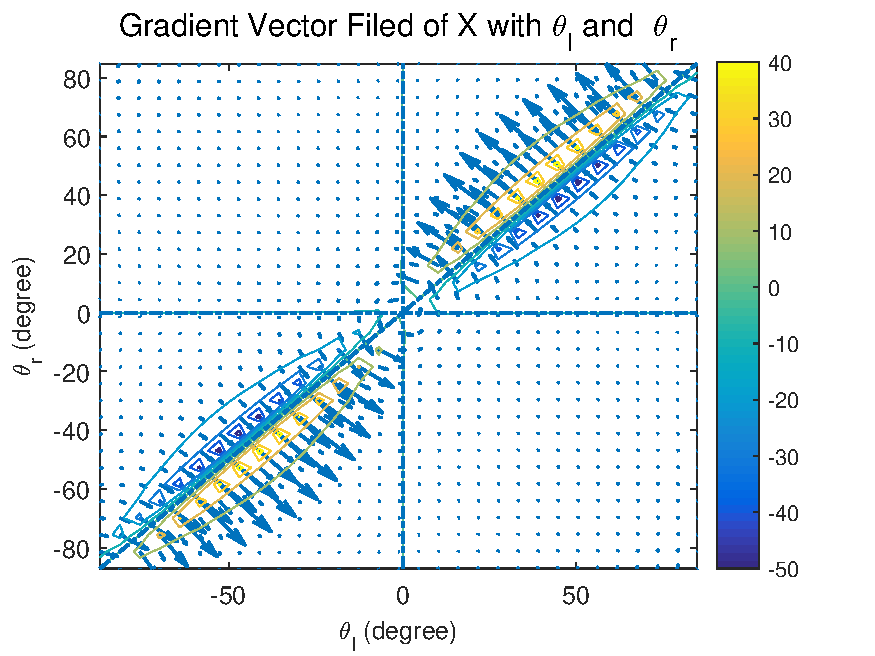
\includegraphics[height=4cm]{Figs/chp03_vision_03_glide_3_x_with_theta_l_r.pdf}
%	}
%	\subfigure[]
%	{
%		\label{fig:ErrorVectorFieldY}
%		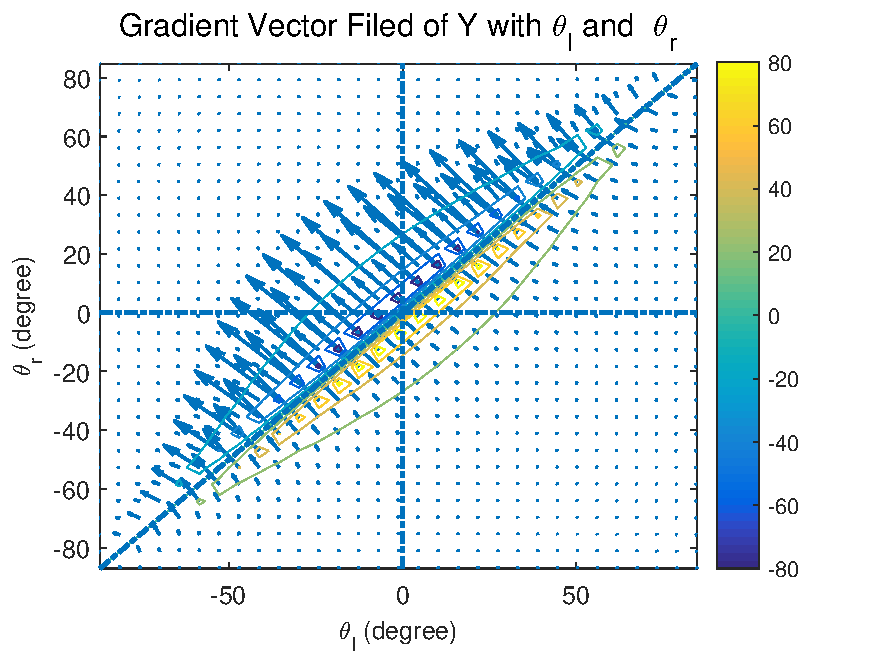
\includegraphics[height=4cm]{Figs/chp03_vision_04_glide_3_y_with_theta_l_r.pdf}
%	}
%	\subfigure[]
%	{
%		\label{fig:ErrorVectorFieldZ}
%		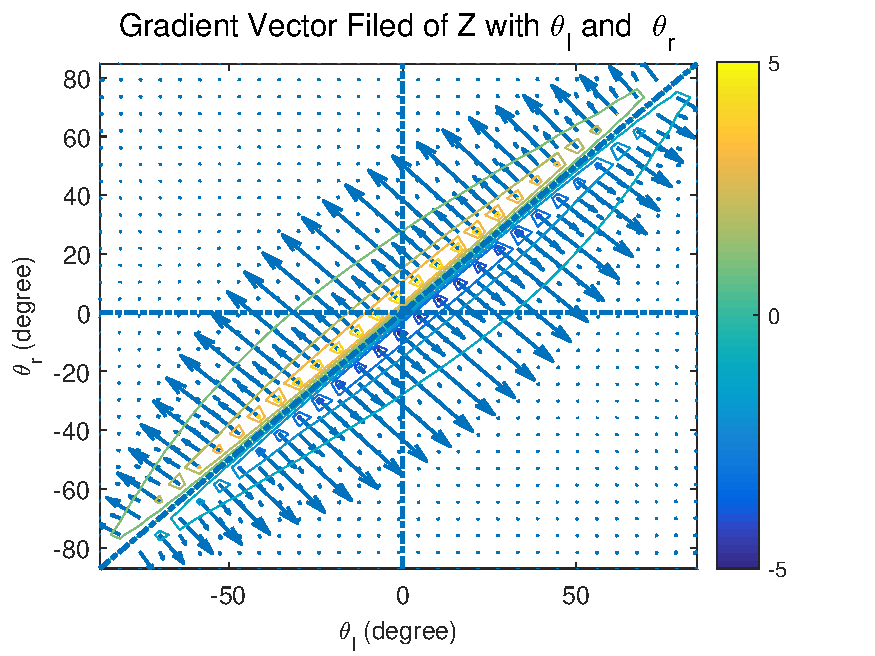
\includegraphics[height=4cm]{Figs/chp03_vision_05_glide_3_z_with_theta_l_r.pdf}
%	}
%	\caption{Vector Field Distribution of $\nabla_{x_M}(\psi_l, \psi_r)$, $\nabla_{y_M}(\psi_l, \psi_r)$, and $\nabla_{z_M}(\psi_l, \psi_r)$}
%\end{figure*}
%
%\begin{figure*}[!tb]
%	\centering
%	\subfigure[]
%	{
%		\label{fig:ErrorVectorFieldX4}
%		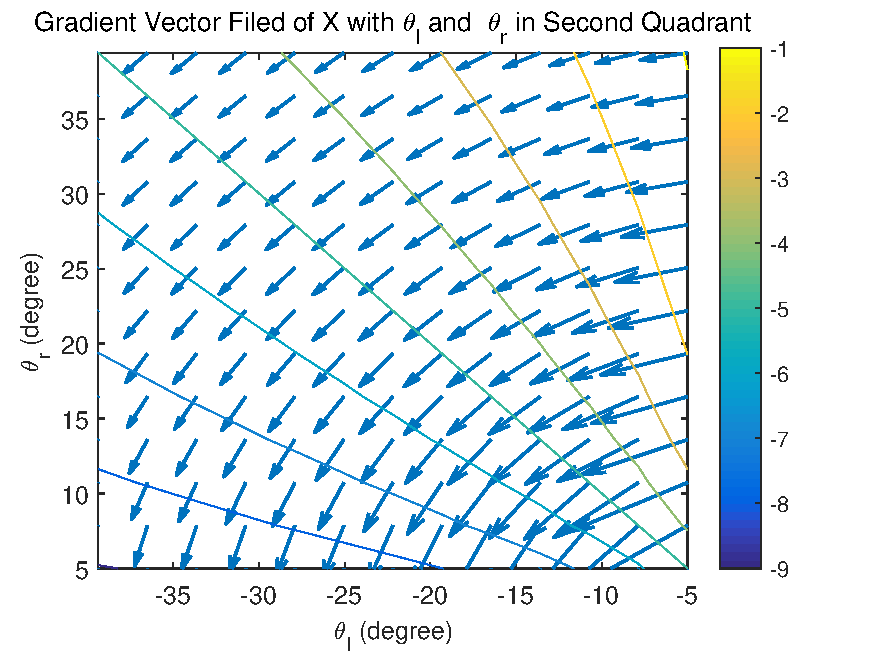
\includegraphics[height=4cm]{Figs/chp03_vision_06_glide_3_x_with_theta_l_r_2_quadrant.pdf}
%	}
%	\subfigure[]
%	{
%		\label{fig:ErrorVectorFieldY4}
%		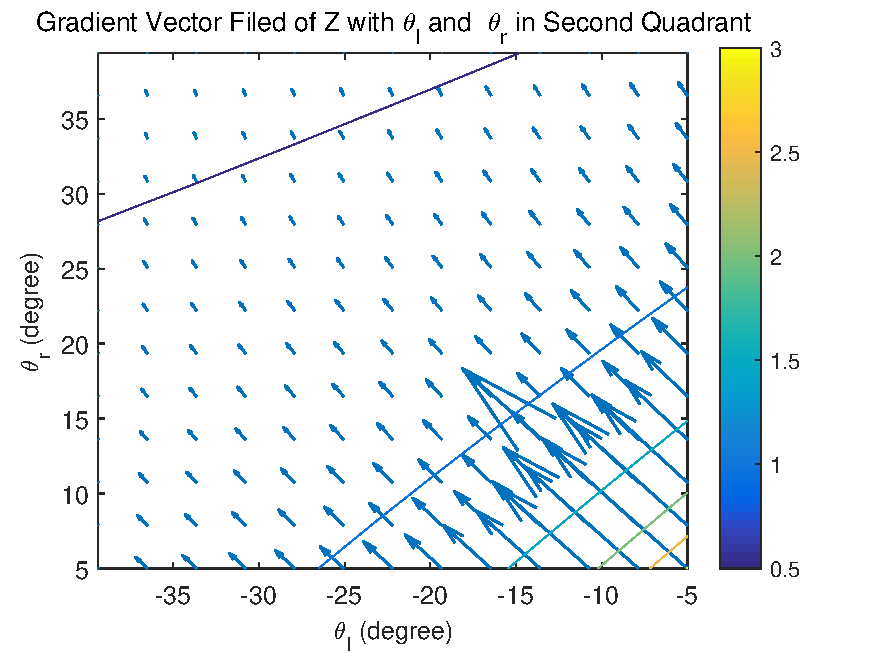
\includegraphics[height=4cm]{Figs/chp03_vision_08_glide_3_z_with_theta_l_r_2_quadrant.pdf}
%	}
%	\subfigure[]
%	{
%		\label{fig:ErrorVectorFieldZ4}
%		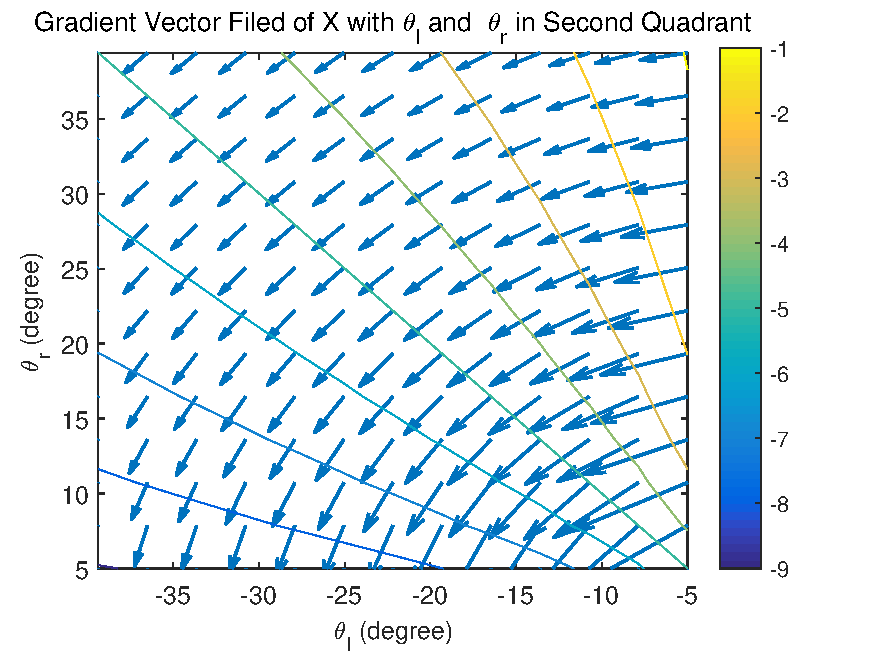
\includegraphics[height=4cm]{Figs/chp03_vision_06_glide_3_x_with_theta_l_r_2_quadrant.pdf}
%	}
%	\subfigure[]
%	{
%		\label{fig:chp03_vision_10_glide_3_gradient_y_2_quadrant}
%		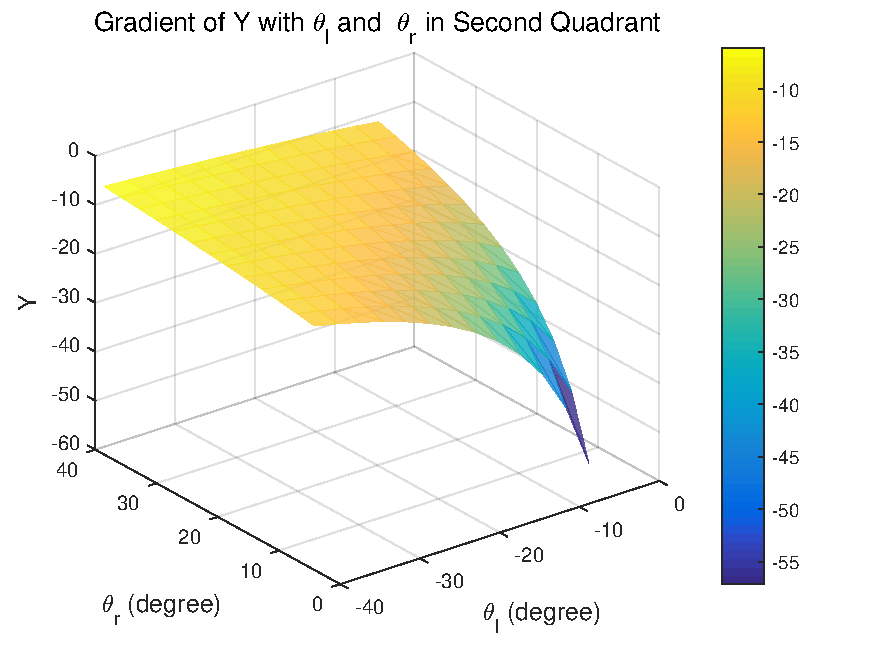
\includegraphics[height=4cm]{Figs/chp03_vision_10_glide_3_gradient_y_2_quadrant.pdf}
%	}
%	\subfigure[]
%	{
%		\label{fig:}
%		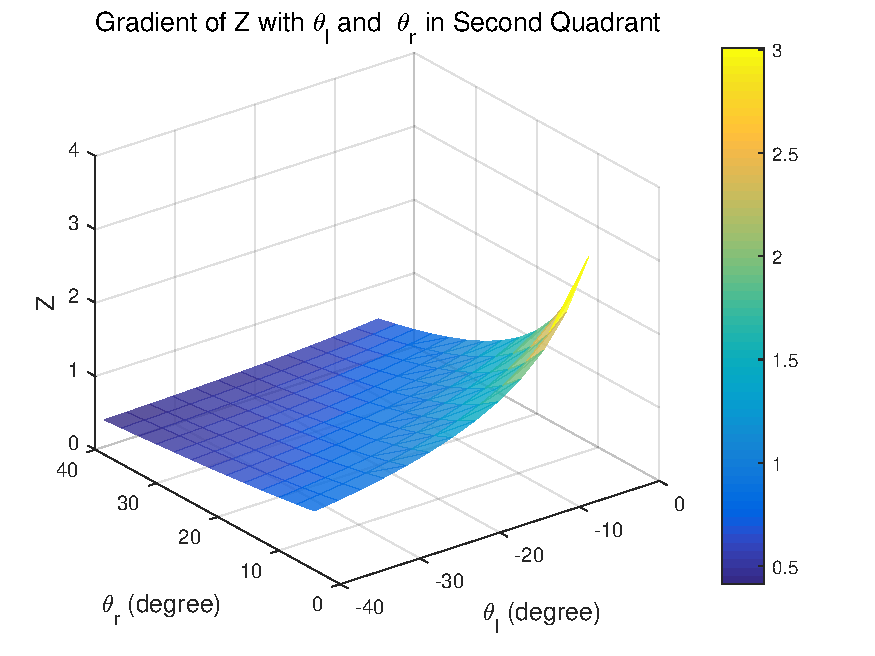
\includegraphics[height=4cm]{Figs/chp03_vision_11_glide_3_gradient_z_2_quadrant.pdf}
%	}	
%	\subfigure[]
%	{
%		\label{fig:chp03_vision_09_glide_3_gradient_x_2_quadrant}
%		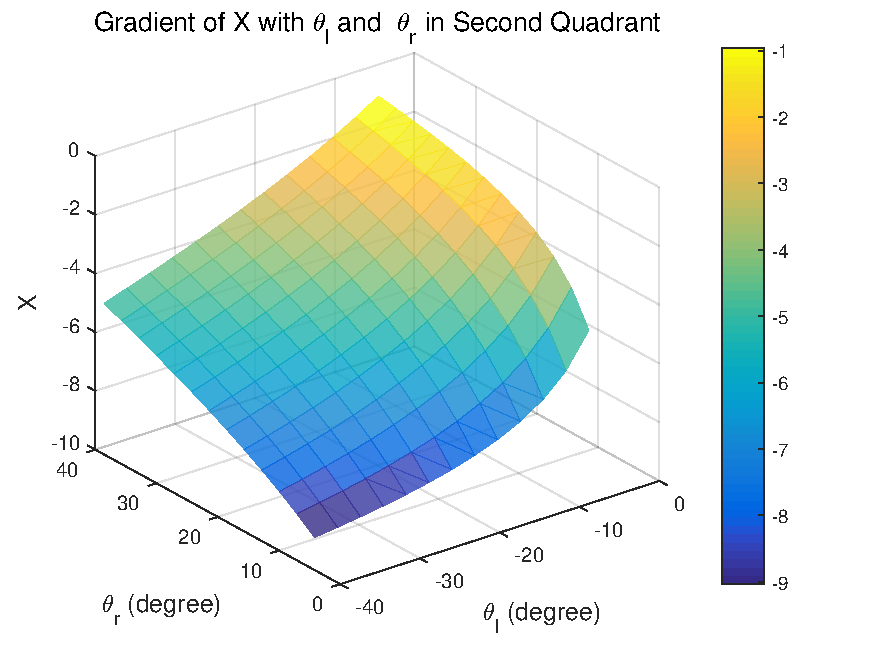
\includegraphics[height=4cm]{Figs/chp03_vision_09_glide_3_gradient_x_2_quadrant.pdf}
%	} 
%	\caption{(a)-(c) Vector Field Distribution of $\nabla_{x_M}(\psi_l, \psi_r)$, $\nabla_{y_M}(\psi_l, \psi_r)$, and $\nabla_{z_M}(\psi_l, \psi_r)$ in Second Quadrant. (d)-(f) Gradient of X, Y, Z with $\theta_l$ and  $\theta_r$ in Second Quadrant}
%\end{figure*}
%
%


\subsection{Practical Analysis}
In theory, $O_lM$ and $O_rM$ should intersect perfectly at one point all the time as shown in Fig. \ref{fig:TheoreticalModel}. Due to the inevitable errors from PTU rotation and tracking algorithms, we estimates the intersecting point by combing the vertical line of two different plane in space.

(1) We set $(x_{ol}, y_{ol}, z_{ol}=(0, 0, 0)$ and $(x_{or}, y_{or}, z_{or}=(D, 0, 0)$ are the optical center of each camera. Assuming that $a_l\neq0$, $b_l\neq0$, $c_l\neq0$ and $a_r\neq0$, $b_r\neq0$, $c_r\neq0$, we obtain the parametric equations of line $O_lM$ and $O_rM$ 
\begin{equation}  
\left \{
	\begin{split}
		&\frac{x-x_{ol}}{a_l} = \frac{y-y_{ol}}{b_l} = \frac{z-z_{ol}}{c_l} = t_l,\\
		&\frac{x-x_{or}}{a_r} = \frac{y-y_{or}}{b_r} = \frac{z-z_{or}}{c_r} = t_r,
	\end{split}
\right.
\end{equation}
\begin{equation}  
\left\{ 
\begin{array}{lll} 
a_l = \cos \phi_l \sin \psi_l\\
b_l = \cos \phi_l \cos \psi_l\\
c_l = \sin \phi_l
\end{array} 
\right.
\end{equation}

\begin{equation} 
\left\{ 
\begin{array}{lll} 
a_r = \cos \phi_r \sin \psi_r\\
b_r = \cos \phi_r \cos \psi_r\\
c_r = \sin \phi_r
\end{array} 
\right.
\end{equation}
where $t_l$, $t_r$ are the parameters for the line $O_lM$ and $O_rM$ separately.
So any point $(x, y, z)$ on each line are usually written parametrically as a function of $t_l$ and $t_r$:
\begin{equation}  
	\left\{ 
	\begin{array}{lll} 
		x_l = a_l t_l + x_{ol} \\
		y_l = b_l t_l + y_{ol} \\
		z_l = c_l t_l + z_{ol}
	\end{array} 
	\right.
\end{equation}

\begin{equation}  
	\left\{ 
	\begin{array}{lll} 
		x_r = a_r l_r + x_{or} \\
		y_r = b_r t_r + y_{or} \\
		z_r = c_r t_r + z_{or}
	\end{array} 
	\right.
\end{equation}

(2) In our situation, $O_lM$ and $O_rM$ are skew lines that these two lines to not be parallel and to not intersect in 3D. Generally, the shortest distance between the two skew lines lies along the line which is perpendicular to both of them. By defining the intersection points of the shortest segment line for each line by $(x_{lp}, y_{lp}, z_{lp}$ and $(x_{rp}, y_{rp}, z_{rp}$, we get the parametric equations
\begin{equation}  
	\left\{ 
	\begin{array}{lll} 
		x_{lp} = a_l t_l + x_{ol} \\
		y_{lp} = b_l t_l + y_{ol} \\
		z_{lp} = c_l t_l + z_{ol}
	\end{array} 
	\right.
\end{equation}
\begin{equation}  
	\left\{ 
	\begin{array}{lll} 
		x_{rp} = a_r l_r + x_{or} \\
		y_{rp} = b_r t_r + y_{or} \\
		z_{rp} = c_r t_r + z_{or}
	\end{array} 
	\right.
\end{equation}


(3) Knowing the position of the intersection points on each line, the distance is calculated by the square Euclidean norm 
\begin{equation}
	J = \|(x_{lp}, y_{lp}, z_{lp}) - (x_{rp}, y_{rp}, z_{rp}) \|_2^2
\end{equation}
The purpose of this method is to minimize this distance. Since two skew lines can always be placed into two parallel planes, we could simplify the problem to finding the shortest distance between the two parallel planes. By taking the partial derivative of the distance function $J$ with respect to $t_l$ and $t_r$ and setting them to 0, the above function can be calculated as:
\begin{flalign}  
	&
	\begin{bmatrix}
		a_l^2 + b_l^2 + c_l^2       & -(a_la_r + b_lb_r + c_lc_r) \\
		-(a_la_r + b_lb_r + c_lc_r) & a_l^2 + b_l^2 + c_l^2 \\    
	\end{bmatrix}	
	\begin{bmatrix}
		t_l \\ 
		t_r 
	\end{bmatrix} \nonumber \\
	&=(x_{ol}-x_{or})
	\begin{bmatrix}
		-a_l \\
		a_r 
	\end{bmatrix}
	+(y_{ol}-y_{or})
	\begin{bmatrix}
		-b_l \\
		b_r 
	\end{bmatrix} \nonumber
	+(z_{ol}-z_{or})
	\begin{bmatrix}
		-c_l \\
		c_r
	\end{bmatrix}.
\end{flalign}

We could then define the matrix as follows:
\begin{flalign} 
\mathbf{H} = 
	\begin{bmatrix} 
		a_l^2 + b_l^2 + c_l^2      & -(a_la_r + b_lb_r + c_lc_r) \\  -(a_la_r + b_lb_r + c_lc_r) & a_l^2 + b_l^2 + c_l^2 \\ 
	\end{bmatrix} 
\end{flalign}
The determinant of this matrix is denoted $\det \mathbf{H} $. When $\det \mathbf{H} = 0$, $MO_l$ and $MO_r$ parallel to each other; when $\det \mathbf{H} \neq 0$, there is an uniqueness vertical line. After solving these equations, the parameter $t_l$ and $t_r$ can be expressed as 

\begin{flalign}
	\left\{
	\begin{aligned}
		t_l=D \frac{\displaystyle a_l (a_l^2 + b_l^2 + c_l^2) - a_r (a_la_r + b_lb_r + c_lc_r)}{\displaystyle (a_lb_r-b_la_r)^2 + (b_lc_r-c_lb_r)^2 + (a_lc_r-c_la_r)^2} \\
		t_r=D \frac{\displaystyle a_l(a_la_r + b_lb_r + c_lc_r)  - a_r (a_l^2 + b_l^2 + c_l^2)}{\displaystyle (a_lb_r-b_la_r)^2 + (b_lc_r-c_lb_r)^2 + (a_lc_r-c_la_r)^2}
	\end{aligned}
	\right.
\end{flalign}
and the two intersecting points of public vertical line are
\small
\begin{equation}
	\left\{ 
	\begin{aligned}
		x_{lp}=a_lD \frac{ a_l (a_l^2 + b_l^2 + c_l^2) - a_r (a_la_r + b_lb_r + c_lc_r)}{ (a_lb_r-b_la_r)^2 + (b_lc_r-c_lb_r)^2 + (a_lc_r-c_la_r)^2} \\
		y_{lp}=b_lD \frac{ a_l (a_l^2 + b_l^2 + c_l^2) - a_r (a_la_r + b_lb_r + c_lc_r)}{ (a_lb_r-b_la_r)^2 + (b_lc_r-c_lb_r)^2 + (a_lc_r-c_la_r)^2} \\
		z_{lp}=c_lD \frac{ a_l (a_l^2 + b_l^2 + c_l^2) - a_r (a_la_r + b_lb_r + c_lc_r)}{ (a_lb_r-b_la_r)^2 + (b_lc_r-c_lb_r)^2 + (a_lc_r-c_la_r)^2}
	\end{aligned}
	\right.
\end{equation}
and 
\begin{equation}
	\left\{
	\begin{aligned}
		&x_{rp}=D \left[ a_r\frac{a_l(a_la_r + b_lb_r + c_lc_r)  - a_r (a_l^2 + b_l^2 + c_l^2)}{ (a_lb_r-b_la_r)^2 + (b_lc_r-c_lb_r)^2 + (a_lc_r-c_la_r)^2}+ 1\right]  \\
		&y_{rp}=b_rD\frac{ a_l(a_la_r + b_lb_r + c_lc_r)  - a_r (a_l^2 + b_l^2 + c_l^2)}{ (a_lb_r-b_la_r)^2 + (b_lc_r-c_lb_r)^2 + (a_lc_r-c_la_r)^2} \\
		&z_{rp}=c_rD \frac{ a_l(a_la_r + b_lb_r + c_lc_r)  - a_r (a_l^2 + b_l^2 + c_l^2)}{ (a_lb_r-b_la_r)^2 + (b_lc_r-c_lb_r)^2 + (a_lc_r-c_la_r)^2}
	\end{aligned}
	\right.
\end{equation}
\normalsize
Further, the optimal point to present point $M$ is the center point of the vertical line segment, which is satisfied the least square method. To reach a more general result, we added weight on the coordinates of each intersecting points and the world coordinate of the target point $M$ is

\begin{flalign}
	\begin{bmatrix}
		x_M \\ 
		y_M \\
		z_M
	\end{bmatrix}
	=w
	\begin{bmatrix}
		x_{lp} \\ 
		y_{lp} \\
		z_{lp}
	\end{bmatrix}
	+(1-w)
	\begin{bmatrix}
		x_{rp} \\ 
		y_{rp} \\
		z_{rp}
	\end{bmatrix}
	, w \in [0,1].
\end{flalign}


The angle between the UAV landing trajectory and the runway area is usually between $5 \degree$ and $7 \degree$. By considering 1 rad normal distributed disturbance (the accuracy of the PTU is $0.006 \degree$), Fig. \ref{fig:Fig06_ErrorSurf2000} illustrates measurement errors of $x_M$, $y_M$ and $z_M$ in case of different points $(x,y) \in S$, where $S= \{ (x,y)| -50 \leq x \leq 50, 20 \leq y \leq 1000 \}$. Obviously, the errors at a considerable  distance are notable, but the incidence of them decline while the aircraft is close to the runway. When the UAV is only 100 m to the landing area, the error of altitude  is about 0.02 m that is dependable for the landing task. 

\begin{figure*}[!th]
	\centering
	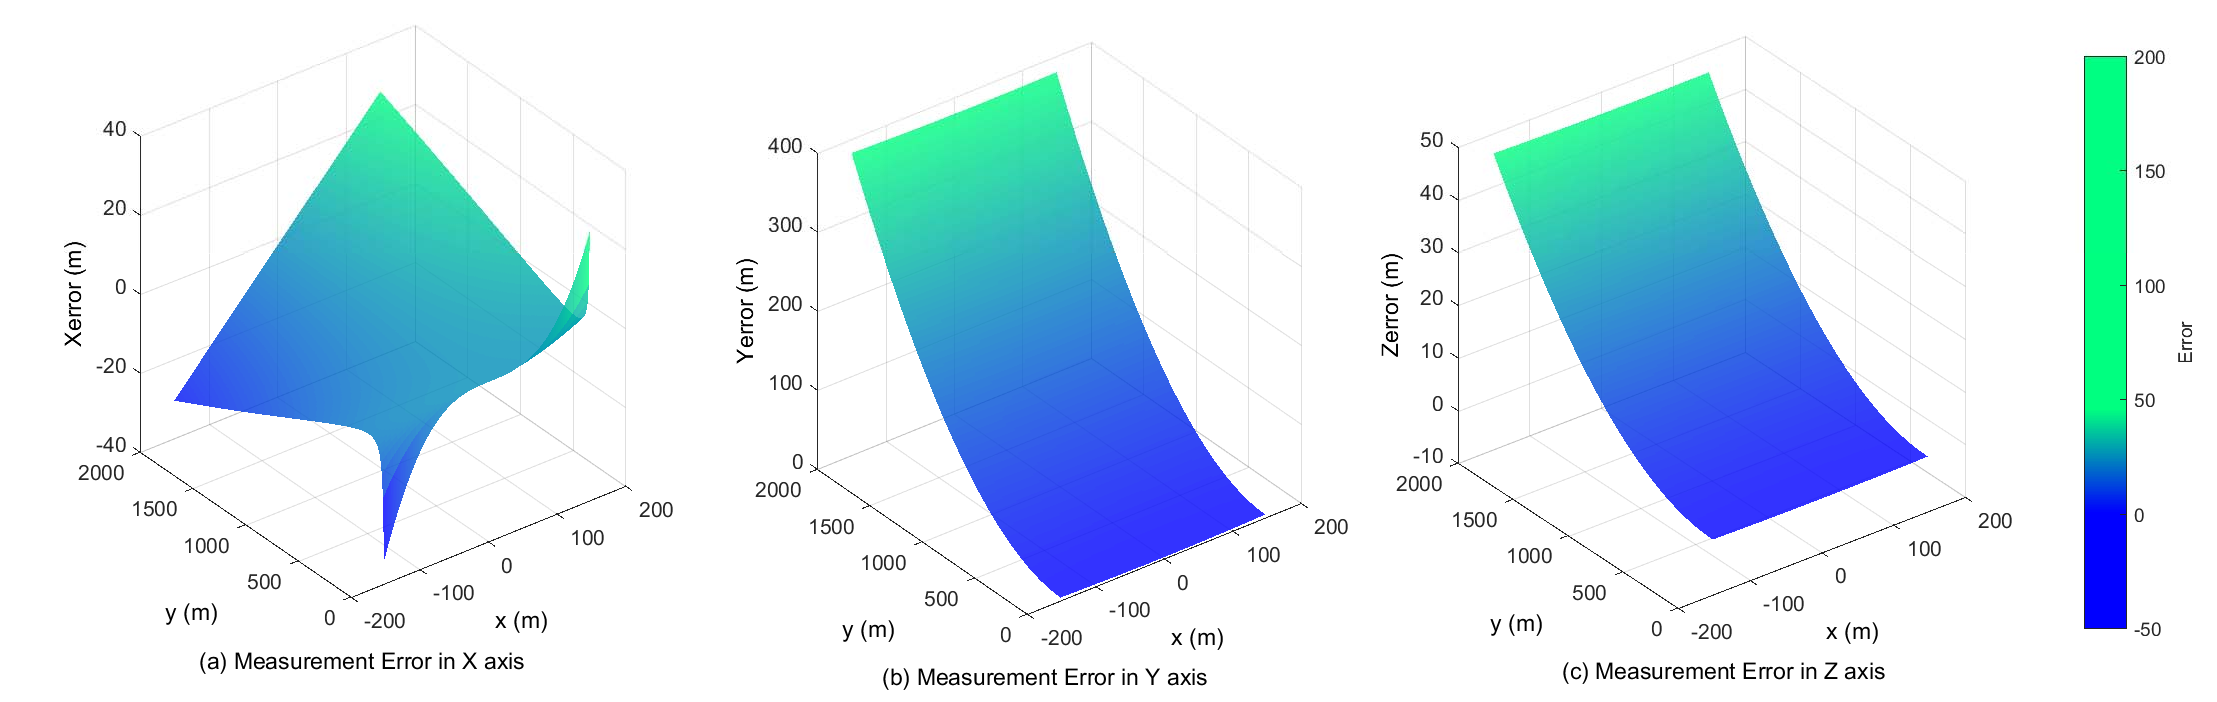
\includegraphics[width=0.8\textwidth]{Figs/Fig06_ErrorSurf2000.pdf}
	\caption{Baseline is $15\ m$. Focus is $100\ mm$. The Mersurement Errors in $X$, $Z$ and $Y$ axis with $2000\ m$.}
	\label{fig:Fig06_ErrorSurf2000}
\end{figure*}

\begin{figure*}[!th]
	\centering
	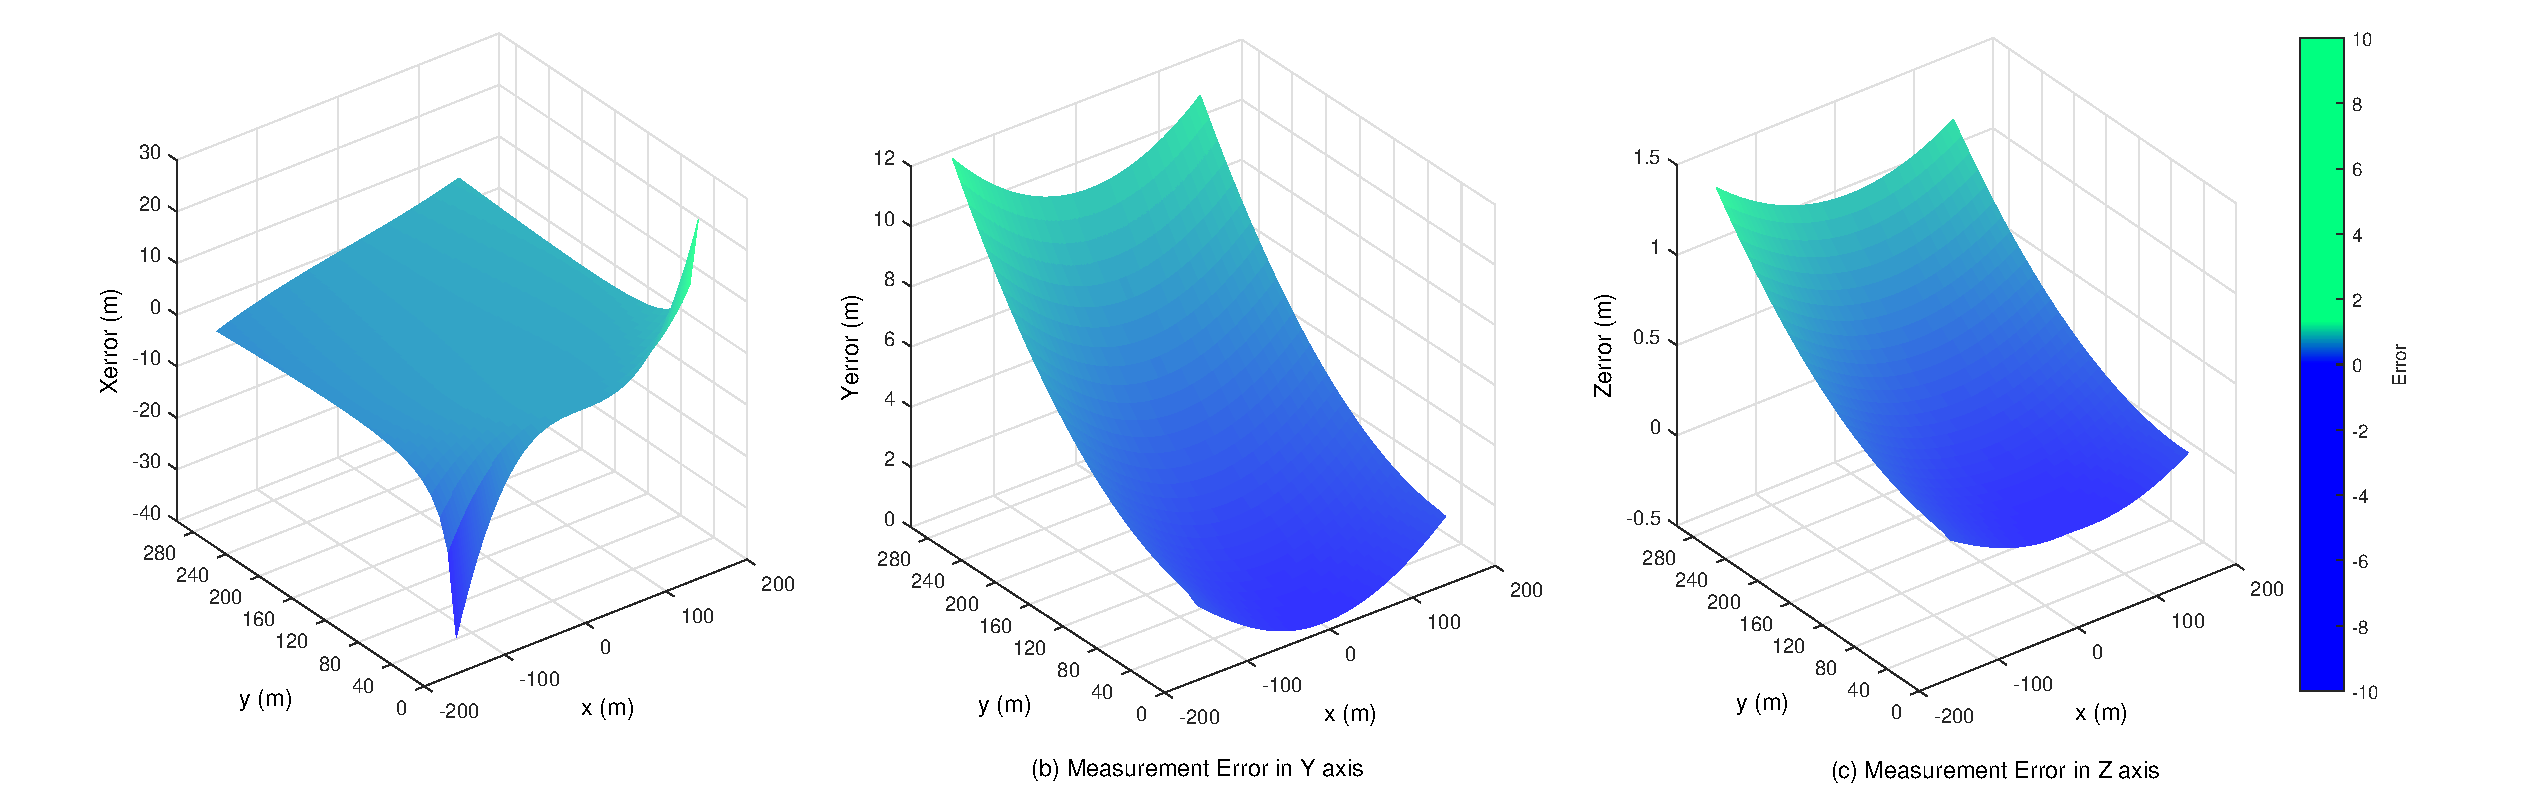
\includegraphics[width=0.8\textwidth]{Figs/Fig07_ErrorSurf200.pdf}
	\caption{Baseline is $15\ m$. Focus is $100\ mm$. The Mersurement Errors in $X$, $Z$ and $Y$ axis with $280\ m$.}
	\label{fig:Fig06_ErrorSurf200}
\end{figure*}
 

\subsection{Implementation}

%TODO: EKF Delayed-state Formulation [NEEC research: Toward GPS-denied landing of unmanned aerial vehicles on ships at sea]

%
%In the basic setup, we separate the vehicle guidance and control into an inner loop and an outer loop, because it is much simpler and well-tested design approach. Because that the inner loop controller is already exist in ??? , we developed an efficient and robust outer guidance loop, which manage the visual information with the on-board sensors.

%The glide slope is the ratio of the distance from the last waypoint to the touchdown point. We generally set this ratio less than 10\% to avoid crashing.


For visible light camera, we selected DFK 23G445 which developed by Imaging Source GmbH shown in Fig. \ref{fig:CameraOnly}. The sensor of this camera is Sony ICX445AQA equipped with GigE interface which has high data transfer rates, typically up to 1000 Mbit/s. This camera has an image resolution of 1280$\times$960 with RGB32 color model, a maximum frame rate of 30 fps. The lens of the vision system we adopted is $100\ mm$, and the baseline is $10\ m$. 
%The ground station, which runs the tracking and localization algorithms, is mainly constituted by ADLINK EOS-1200 PC, which sends relative position and records GNSS data from UAV as ground truth.  This product is a rugged and compact system equipped with Intel Core i7 2.1 GHz processor and 8 GB DDR3. 


\begin{figure}[!tb]
	\centering
	\subfigure[]
	{
		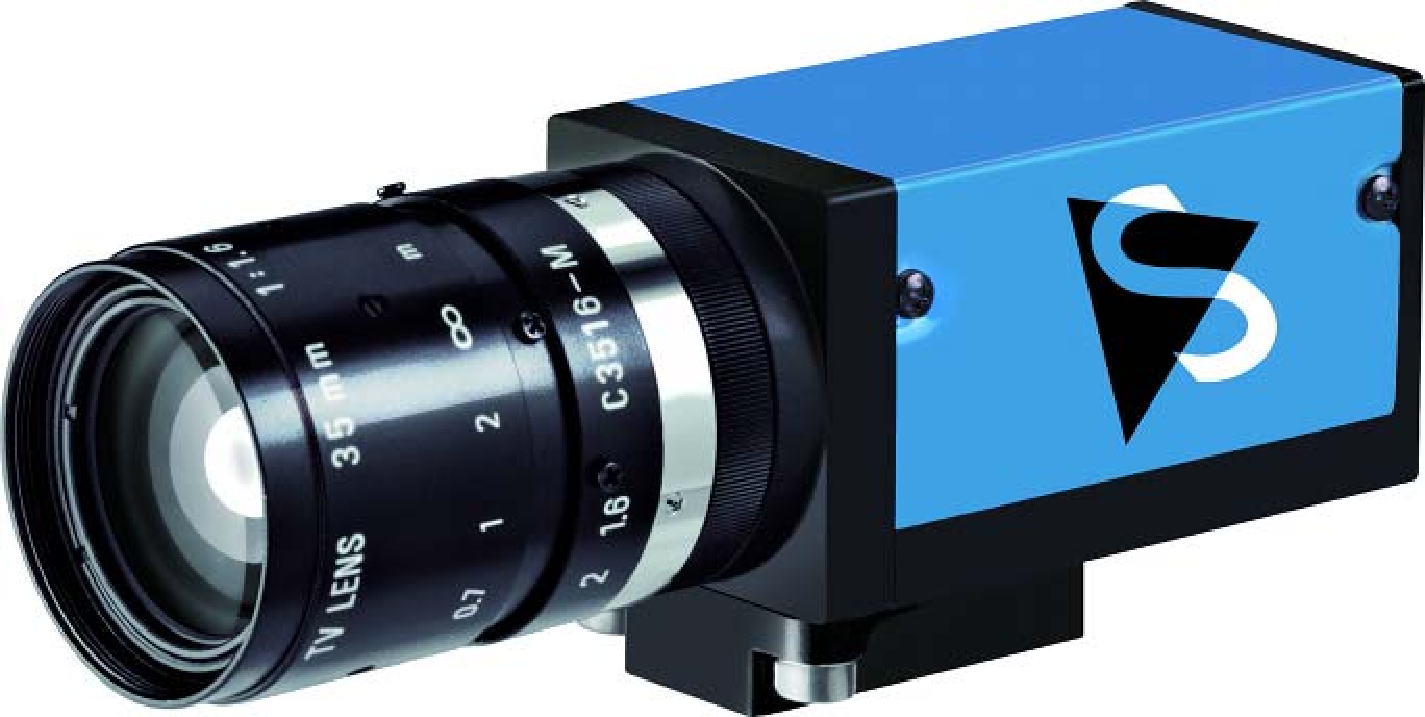
\includegraphics[height=1.6cm]{Figs/CameraOnly.pdf}
		\label{fig:CameraOnly}
	}
	\subfigure[]
	{
		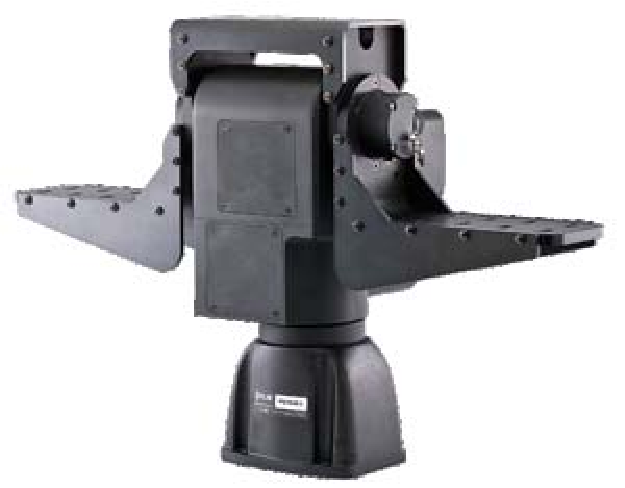
\includegraphics[height=2.6cm]{Figs/PTU_D300E.pdf}
		\label{fig:PTU_D300E}
	}
	\caption{(a) DFK 23G445 Camera (b) PTU-D300E}
\end{figure}

To extend the field of view, we adopted precision PTU to actuate the camera. PTU-D300E (see Fig. \ref{fig:PTU_D300E} is a high performance product from FLIR. Its pan/tilt speeds up to $50\degree/second$ with the position resolution of $0.006\degree$. Moreover, it is a user programmable product integrating Ethernet  and RS-232 interface. The real-time command interface supports advanced applications such as video tracking. We set up the camera on the top bracketing, and the assembled individual vision system is illustrated in Fig. \ref{fig:SystemStructure}. 

%For short-baseline configuration, cameras were setup on one PTU (Fig. \ref{fig:chp08_18_ground_short_ptus}) and the system should mount on the center line of the runway. However, this system has limited range for UAV detection. According to our discussion in last section, we could also fix the cameras with separated PTU on the both sides of the runway, as shown in Fig. \ref{fig:SystemOutsideRealPic}, so the landing aircraft can be locked by our system around $1\ km$.

%\begin{figure}[!ht]
%	\centering
%	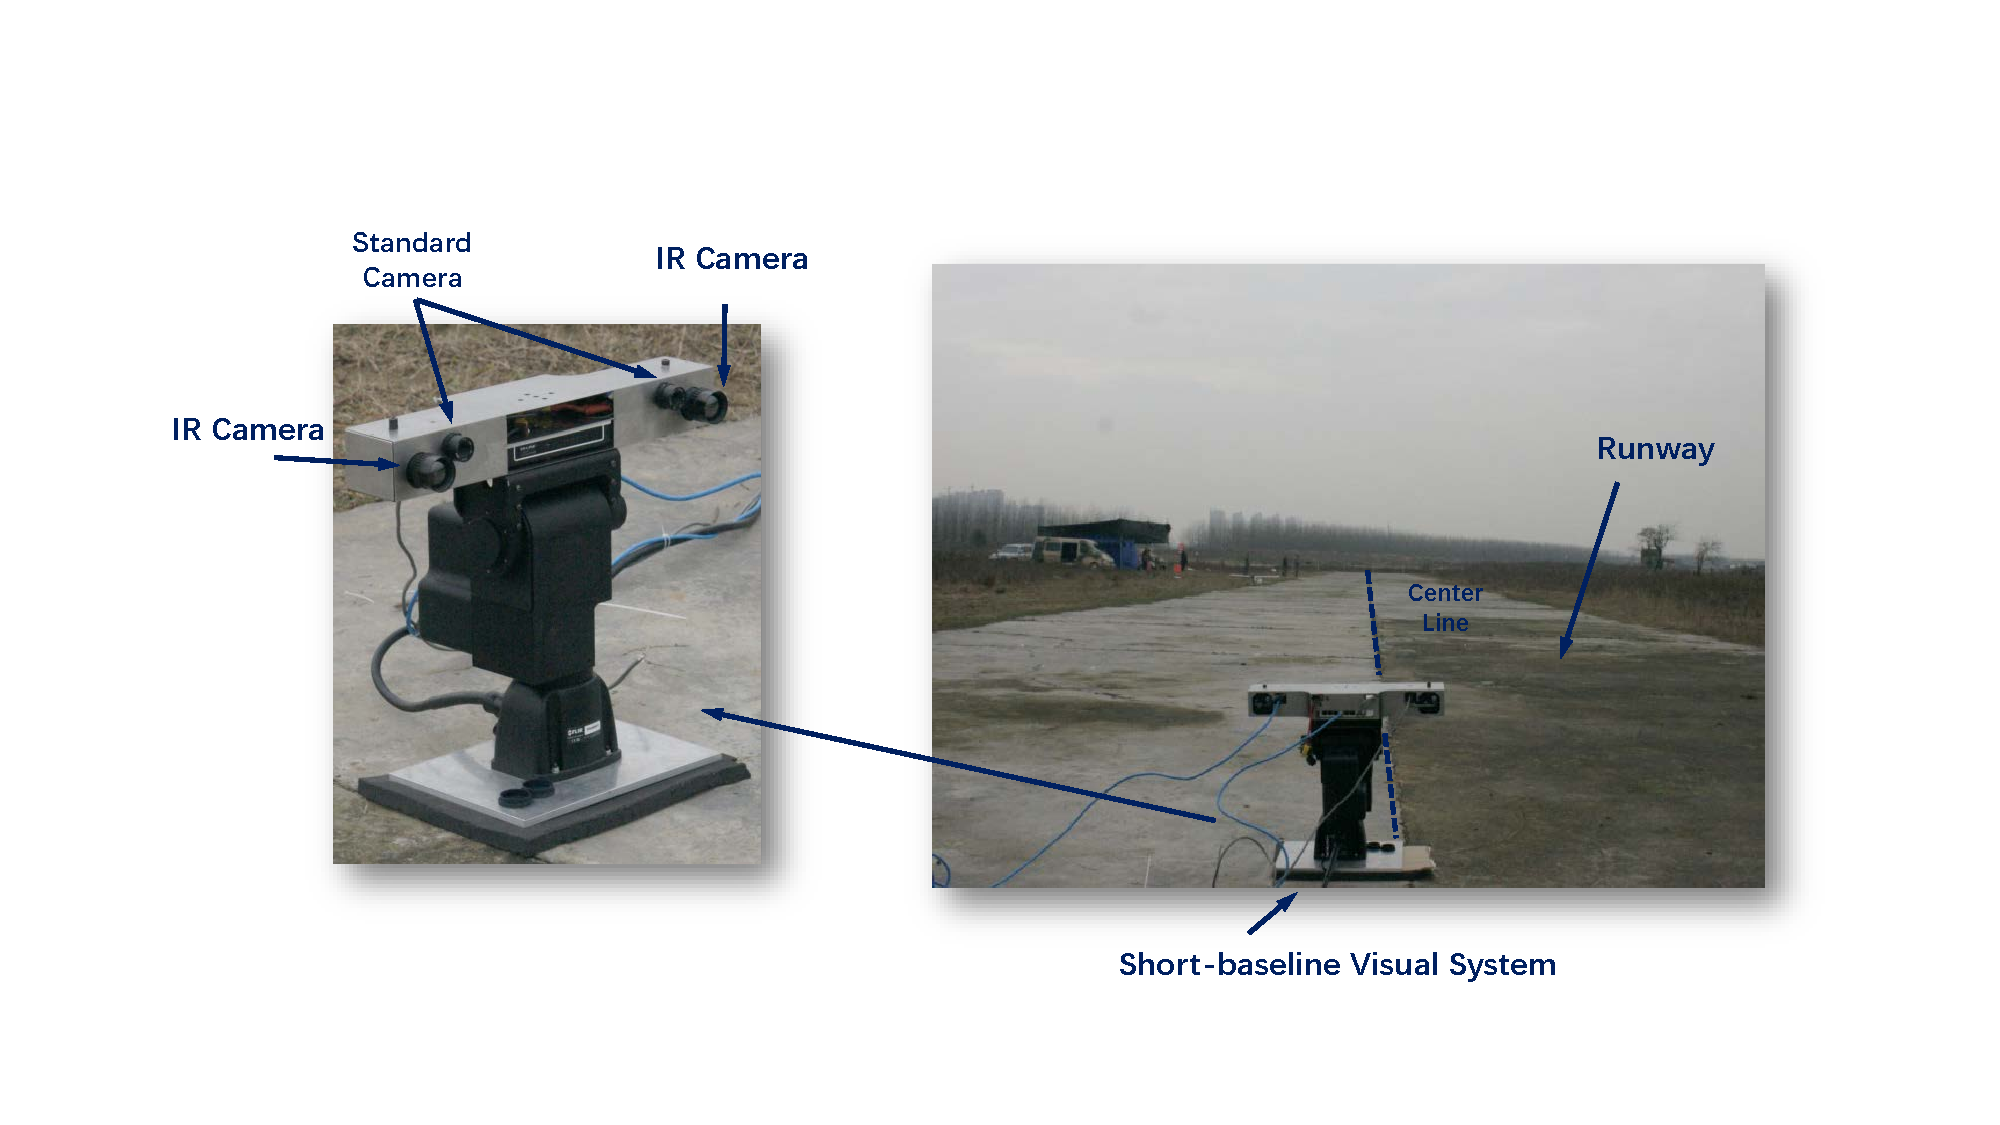
\includegraphics[width=0.6\textwidth]{Figs/chp08_18_ground_short_ptus.pdf}	
%	\caption{Short-baseline Ground System}
%	\label{fig:chp08_18_ground_short_ptus}
%\end{figure}


%
%\begin{figure}[!tb]
%	\centering
%	\subfigure[]
%	{
%		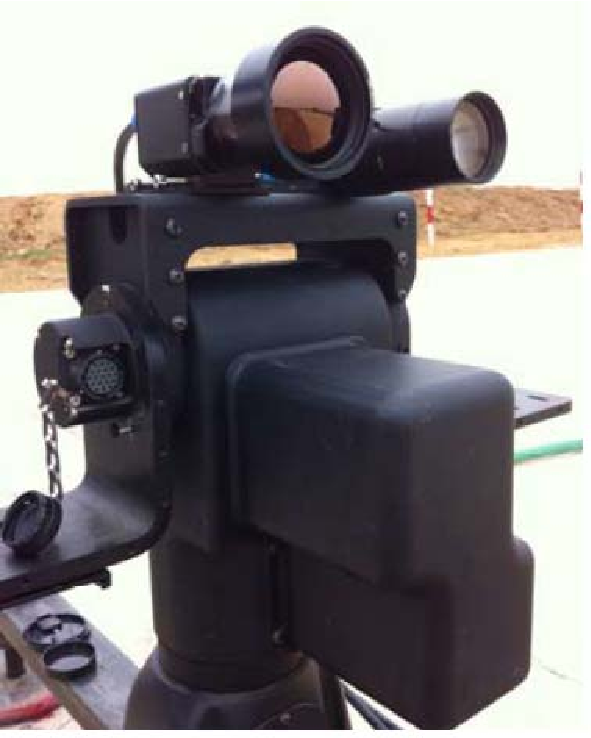
\includegraphics[height=4cm]{Figs/PTUwithCamera.pdf}
%		\label{fig:PTUwithCamera}
%	}
%	\subfigure[]
%	{
%		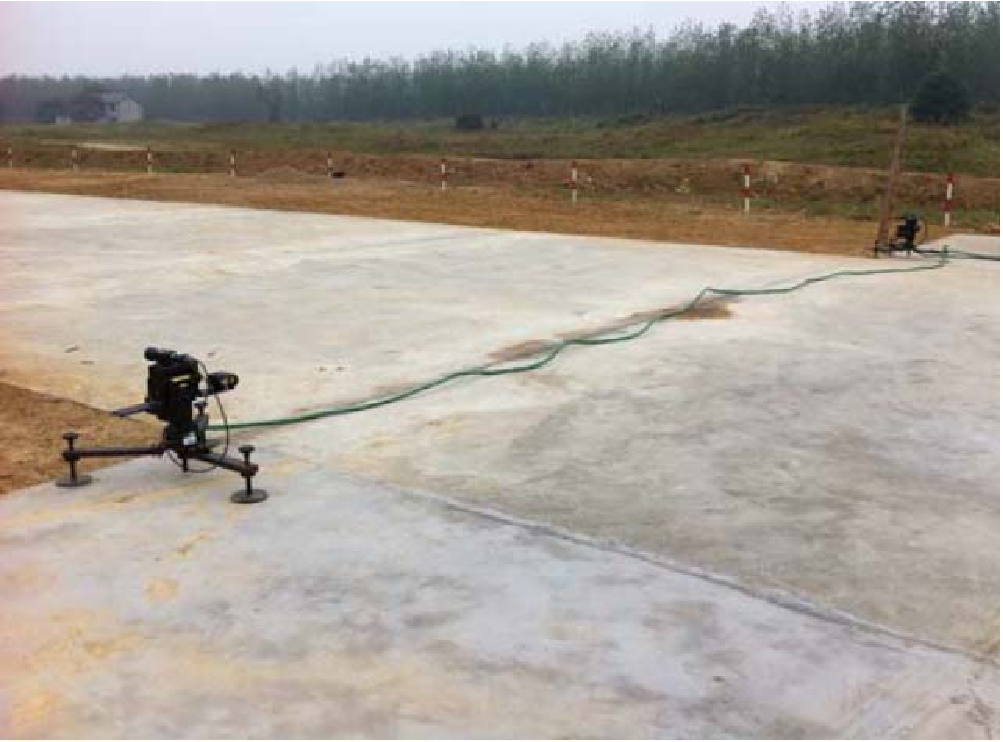
\includegraphics[height=4cm]{Figs/SystemOutsideRealPic.pdf}
%		\label{fig:SystemOutsideRealPic}
%	}
%	\caption{(a) Assembled vision system. (b) The setup of the visual system.}
%\end{figure}
%%
%
%Proper control of the PTU system can keep the landing target in the field of view of the camera. Figure \ref{fig:Fig02_ImagePlaneOnly} shows the focal frame ($f_x$, $f_y$, $f_z$), constructed about the focal point of the camera, $F$, and the image plane is ($u, $v).  In our application, we assume that the axis of rotation for pan and tilt coincide with the two optical center. The rotation angles are defined as $(\phi, \theta, \psi)$. The angle $\psi$, as shown in Fig. \ref{fig:Fig02_ImagePlaneOnly}, between the target and the $f_y$ axis is calculated by
%\begin{equation}
%	tan(\phi)=\frac{v-v_0}{l}
%\end{equation}
%\begin{equation}
%	tan(\psi)=\frac{u-u_0}{f}
%\end{equation}
%where $(u_0, v_0)$ is the principle point in pixel, $(u, v)$ is the current target coordinate in pixel, $f$ is the focus in pixel and $l$ is the direct distance from the optical center to the projected point of the target onto $u$ axis. It can be inferred from the Fig \ref{fig:Fig02_ImagePlaneOnly} that
%\begin{align} \label{eq:FOV_TILT}
%	\phi &=f(v, v_0, w_v, \alpha_{FOV_{tilt}}) \\
%	&=atan(v-v_0, \frac{w_v}{2}cot \frac{\alpha_{FOV_{tilt}}}{2})
%\end{align}
%\begin{align} \label{eq:FOV_PAN}
%	\psi &=f(u, u_0, w_u, \alpha_{FOV_{pan}}) \\
%	&=atan(u-u_0, \frac{w_u}{2}cot\frac{\alpha_{FOV_{pan}}}{2})
%\end{align}
%where $w_u$ and $w_v$ are size of image plane in pixel, $\alpha_{FOV_{pan}}$ and $\alpha_{FOV_{tilt}}$ are the filed of view in radians. There is no rotation around Y axis, so $\theta = 0$. Let the target coordinate be at $(u_1, v_1)$, the desired location be at $(u_2, v_2)$. Using equation (\ref{eq:FOV_TILT} and (\ref{eq:FOV_PAN}, the resulting of pan and tilt compensation to keep the target to the desired location in the image plane is given by
%\begin{equation}
%	\Delta\phi=f(v_1,v_0,w_v, \alpha_{FOV_{tilt}}-f(v_2,v_0, w_v, \alpha_{FOV_{tilt}})
%\end{equation}
%\begin{equation}
%	\Delta\psi=f(u_1,u_0,w_u, \alpha_{FOV_{pan}}-f(u_2,u_0, w_u, \alpha_{FOV_{pan}})
%\end{equation}
%Generally, we let the desired location be the principle point in order to keep the target projecting at the center area of the image plane.

The overall architecture of the separated stereo system and its connections and data flows are shown in Fig. \ref{fig:SystemStructure}. Each vision unit work independently and transfers the results of image processing and PTU status to the navigation computer which calculates the estimated relative position of the UAV. Since the ground station judging the switch from GNSS-aid method to vision-aid method, the auto pilot guided UAV based on the properly data received by XTend modem. 

\begin{figure}[!tb]
	\centering
	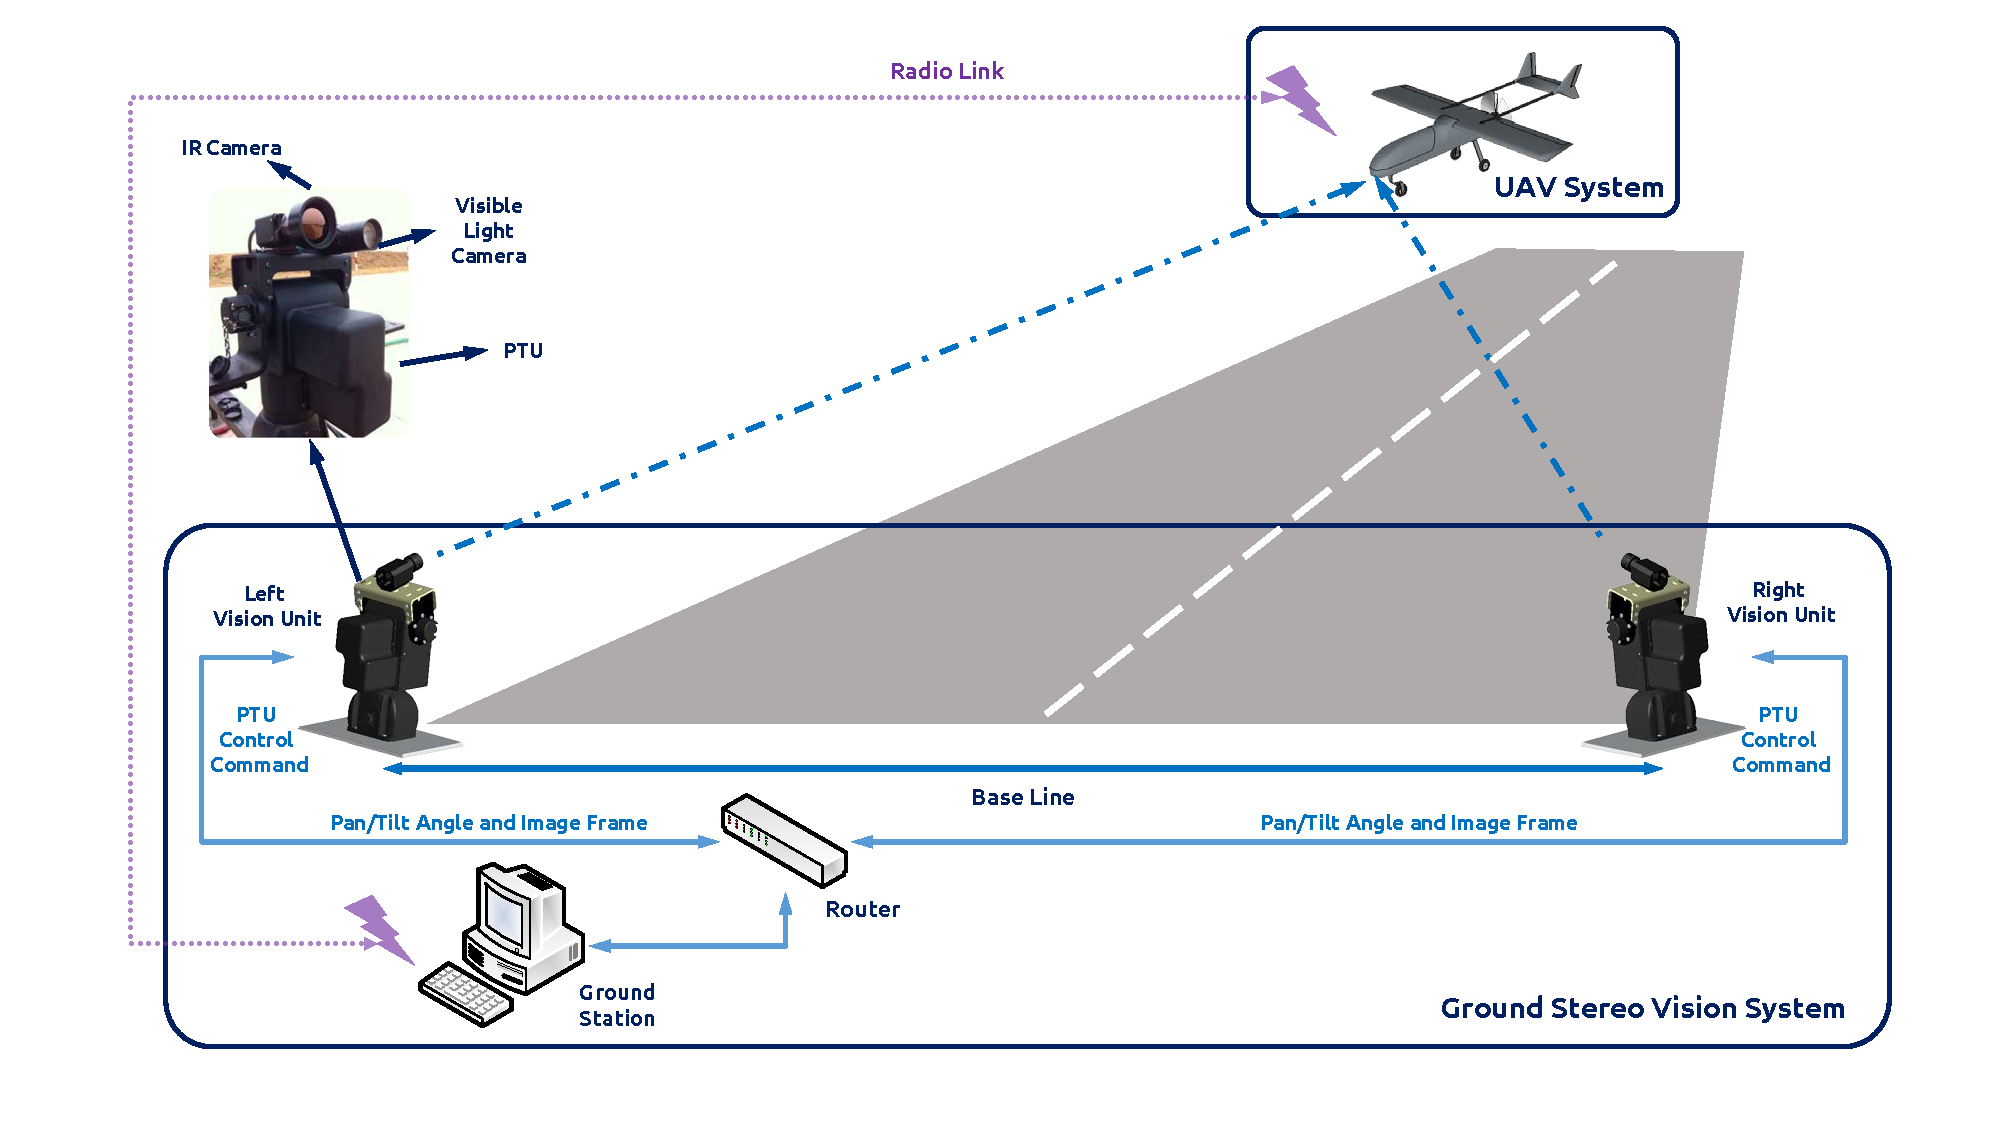
\includegraphics[width=\textwidth]{Figs/SystemStructure2.pdf}
	\caption{Architecture of the system.}
	\label{fig:SystemStructure}
\end{figure}




\section{Tracking and Localization Algorithms}
To keep the camera on the PTU pointing to the target closely, we designed a   vision tracking framework based on TLD and active contour algorithm. Also, the camera rotation angle in pan and tilt axis, which can be received through the serial port from PTU, can also improve the tracking accuracy. Fig. \ref{fig:sci01_tracking_framework} shows the tracking framework.

\begin{figure*}[!th]
	\centering
	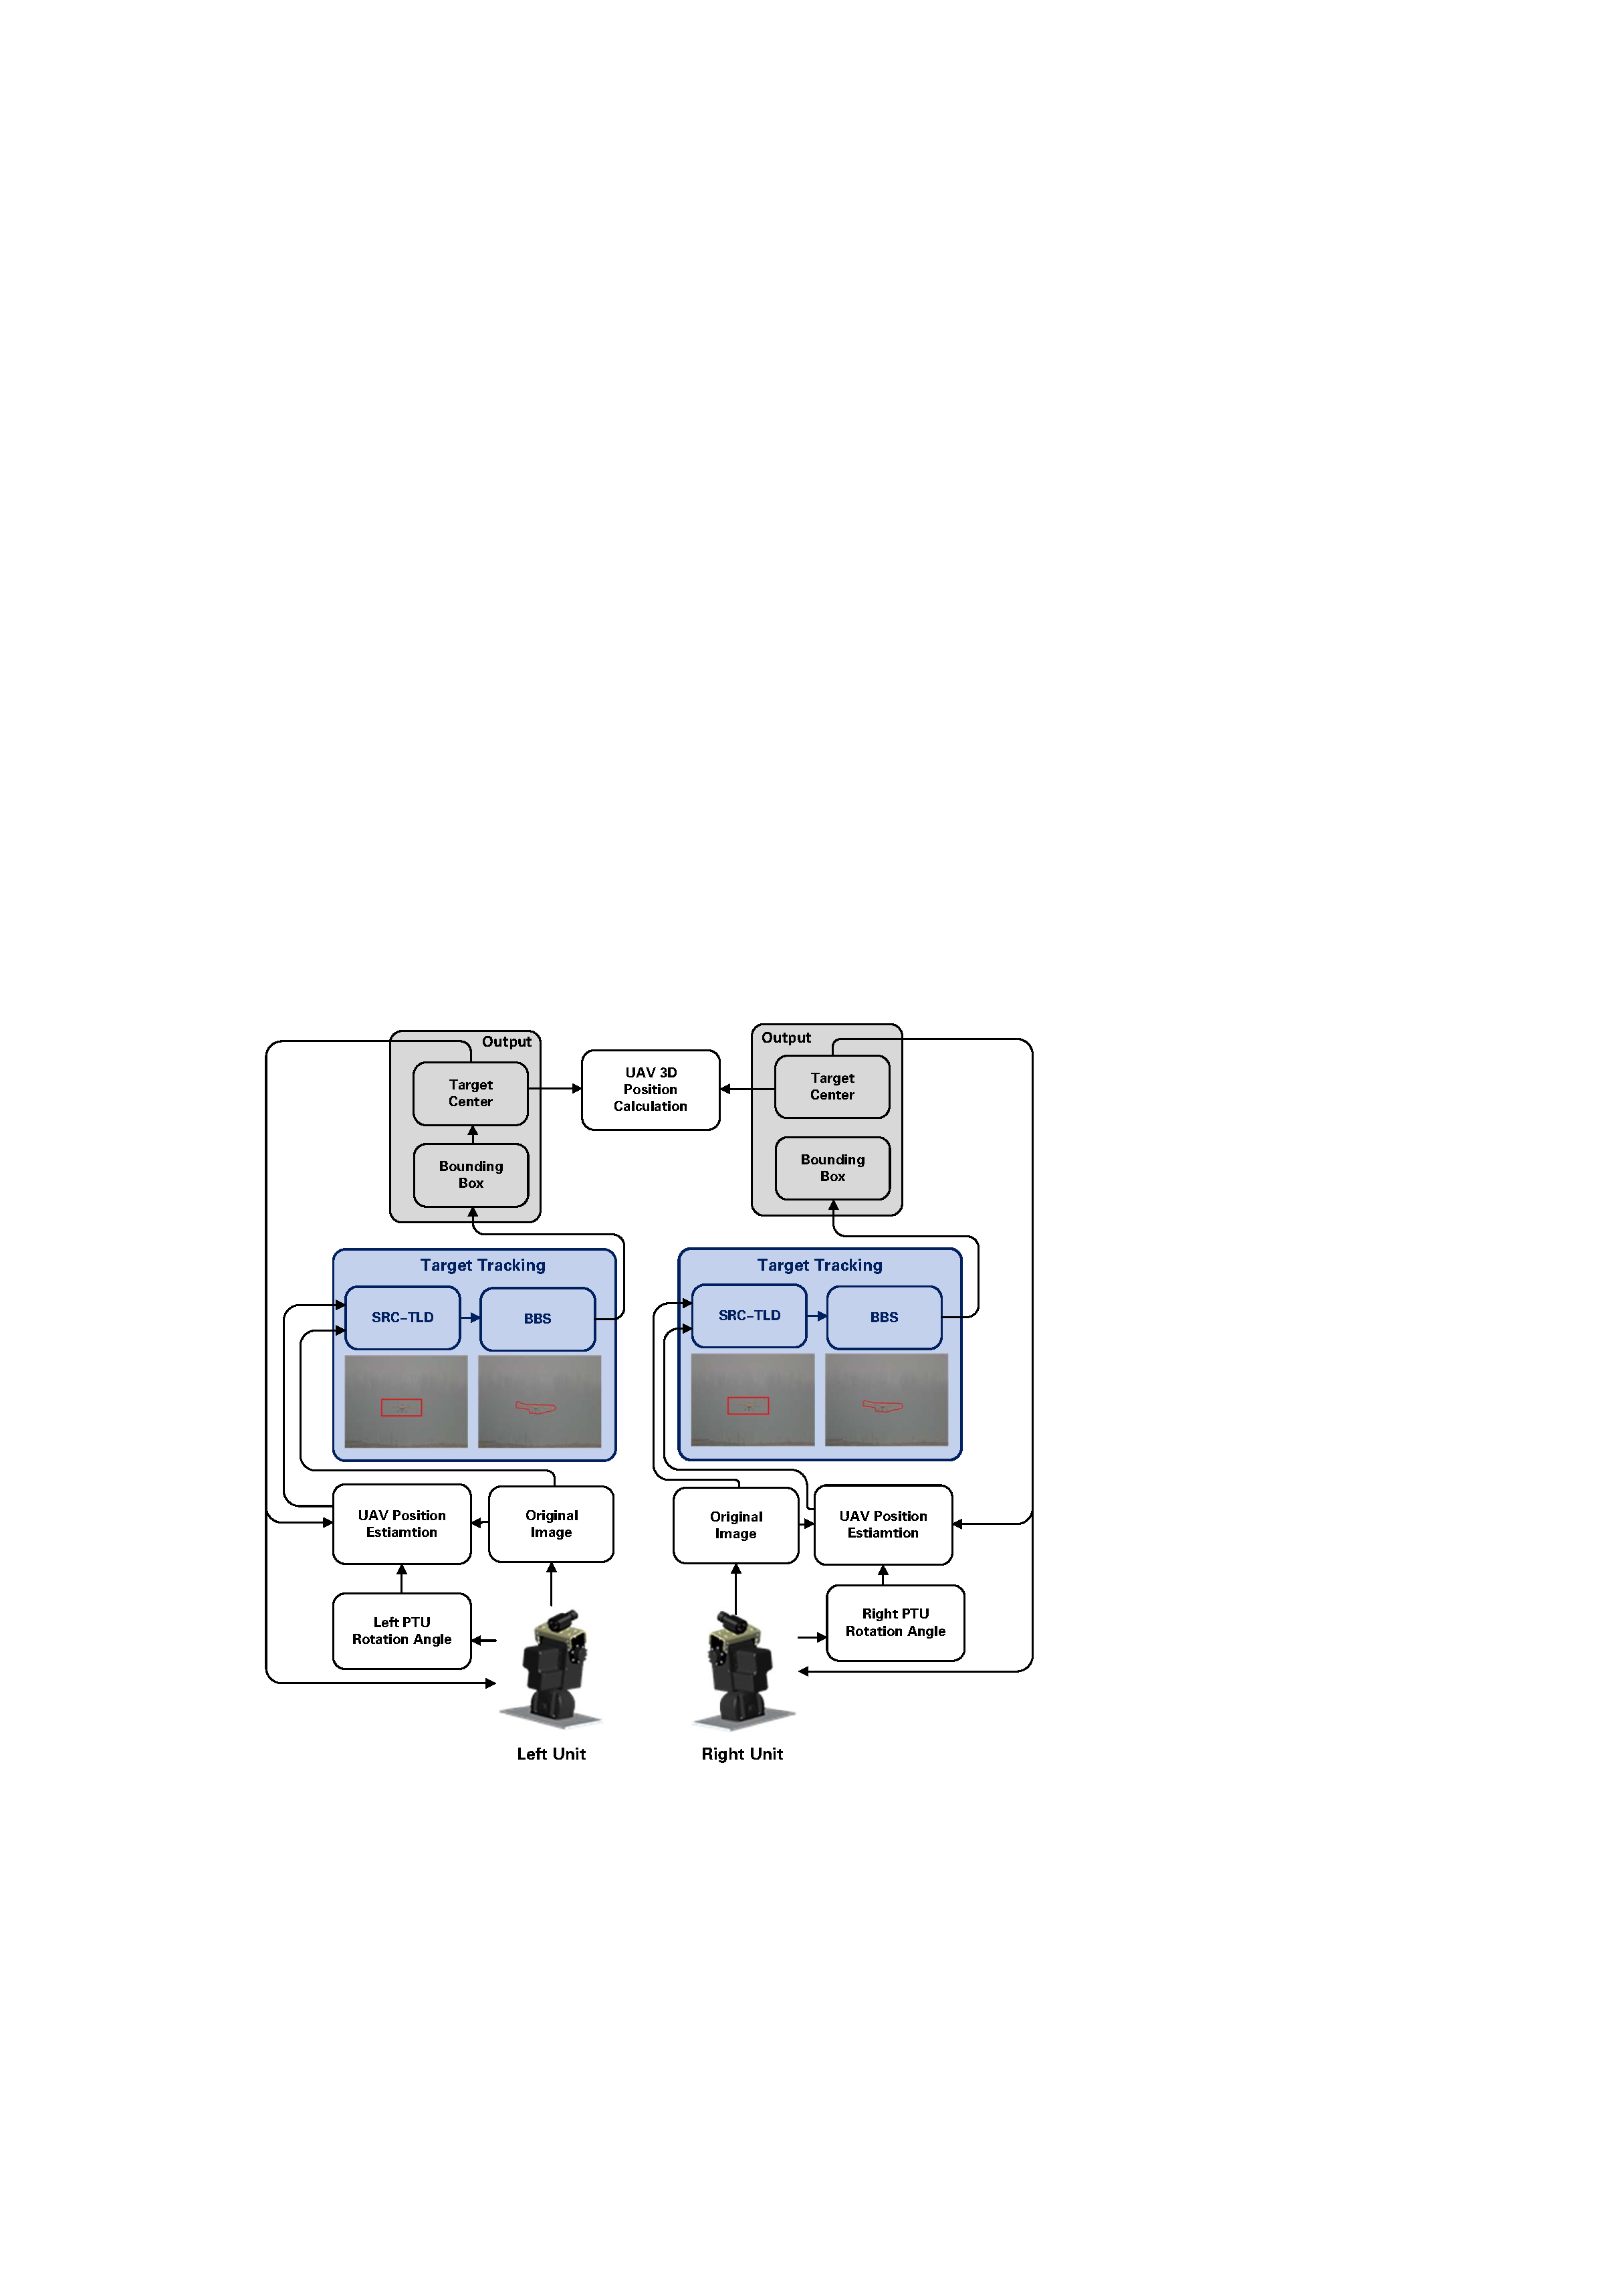
\includegraphics[width=0.9\textwidth]{Figs/sci01_tracking_framework2.pdf}	
	\caption{PTU-based UAV Tracking Framework}
	\label{fig:sci01_tracking_framework}
\end{figure*}

\subsection{SRC-TLD Algorithm}
TLD is an adaptive tracking-by-learning approach, which tracks by learning the appearance of the target - using the online learned classifier to detect the object during the progress. It is consist of three components: 
\begin{itemize}
	\item Tracker is based on Lucas-Kanade method, which could track the target frame by frame and generate examples for learning components.
	
	\item Detector is to solve the classification problem based on random forest algorithm.
	
	\item Learning uses trackers to generate positive and negative samples which is mainly based on P-N Learning mechanisms. Also it update the inner model of the detector.
\end{itemize}
All of these three components runs independently during the calculation.

To describe the target, we compare the intensity values of several pixels.  An example of five-pair feature calculation for a single ferns shows in Fig.\ref{fig:01_TLD_Code}. The random pairs method selects the five different location randomly and the result of each of these comparisons is interpreted as a binary digit, 10011. When written in decimal form, we get 19. A probability could be obtained combing the other training data set.

However, the random pairs is suitable for the target, which could fully filled the subwindow, such as in face or pedestrian detection scenes. This kind of randomness could retrieve the feature of the target and adapts the variance during the tracking process. For fixed-wing MAV, this type of target only displays in the narrow part of the subwindow as shown in light yellow rectangle. Especially the wings of the MAV seems to be a single line when it is far away from the runway. The general randomness lose the kernel feature of the target occasionally, so we set one pixel of each pair randomly only in the yellow rectangle and the other pixel located in the rest part of the subwindow.  We named this process Semi-random Coding (SRC). 

\begin{figure}[!th]
	\centering
	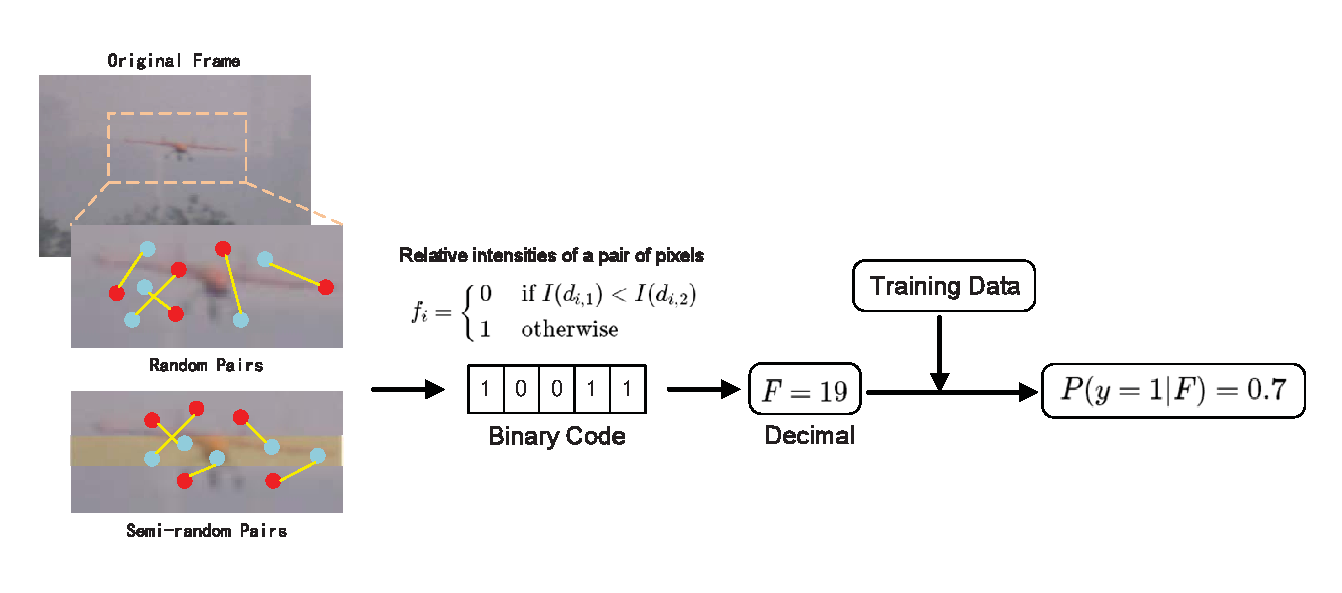
\includegraphics[width=0.8\textwidth]{Figs/01_TLD_Code.pdf}
	\caption{ We compare the intensities of different pairs for each image to get the binary code, then store it as decimal. Random pairs are generated randomly through the whole image plane. For semi-random pairs, one of the point is located randomly in the light yellow filed and the other point is generated randomly at the rest part.}
	\label{fig:01_TLD_Code}    
\end{figure}


\subsection{Bounding Box Shrinking Algorithm}
In order to enhance the localization accuracy, we need to detect the center of aircraft more precisely. However, the target center of SRC-TLD is the centroid of the bounding box which is not always true when the UAV was turning during the landing process. The left image of Fig.\ref{fig:chp04_07_active_contour_demo} shows the standard results of SRC-TLD results. The green bouding box is the ground truth, and the red one is achieved from the SRC-TLD method. Active contour algorithm is one of the choice to converge the predefined rectangle to the UAV main body as shown in the right image of Fig.\ref{fig:chp04_07_active_contour_demo}.

Some previous works \cite{betser2004automatic} and \cite{sattigeri2007vision}, demonstrated that active contours are autonomous processes which employ image coherence in order to track various features of interest over time. A book \cite{blake1998active}and the references therein described snakes fit very spontaneously into a control framework. The starting point of Level Set Method is  \cite{368173}, \cite{Caselles1993} in which an active contour model founded on the level set formulation of the Euclidean curve shortening equation is proposed. Specifically, the model is:
\begin{equation} \label{eq:BasicModel}
\frac{\partial \Psi}{\partial t} = \phi(x,y) \left\|\nabla\Psi\right\| (\texttt{div}(\frac{\nabla \Psi}{\left\|\nabla\Psi\right\|})+\nu) 
\end{equation}
the function $ \phi(x,y) $ depends on the given image and is used as a ``stopping term''. Generally the term  $ \phi(x,y) $ is selected to be small near an intensity-based edge and acts to stop evolution when the contour gets close to an edge.

\begin{figure}[!th]
	\centering
	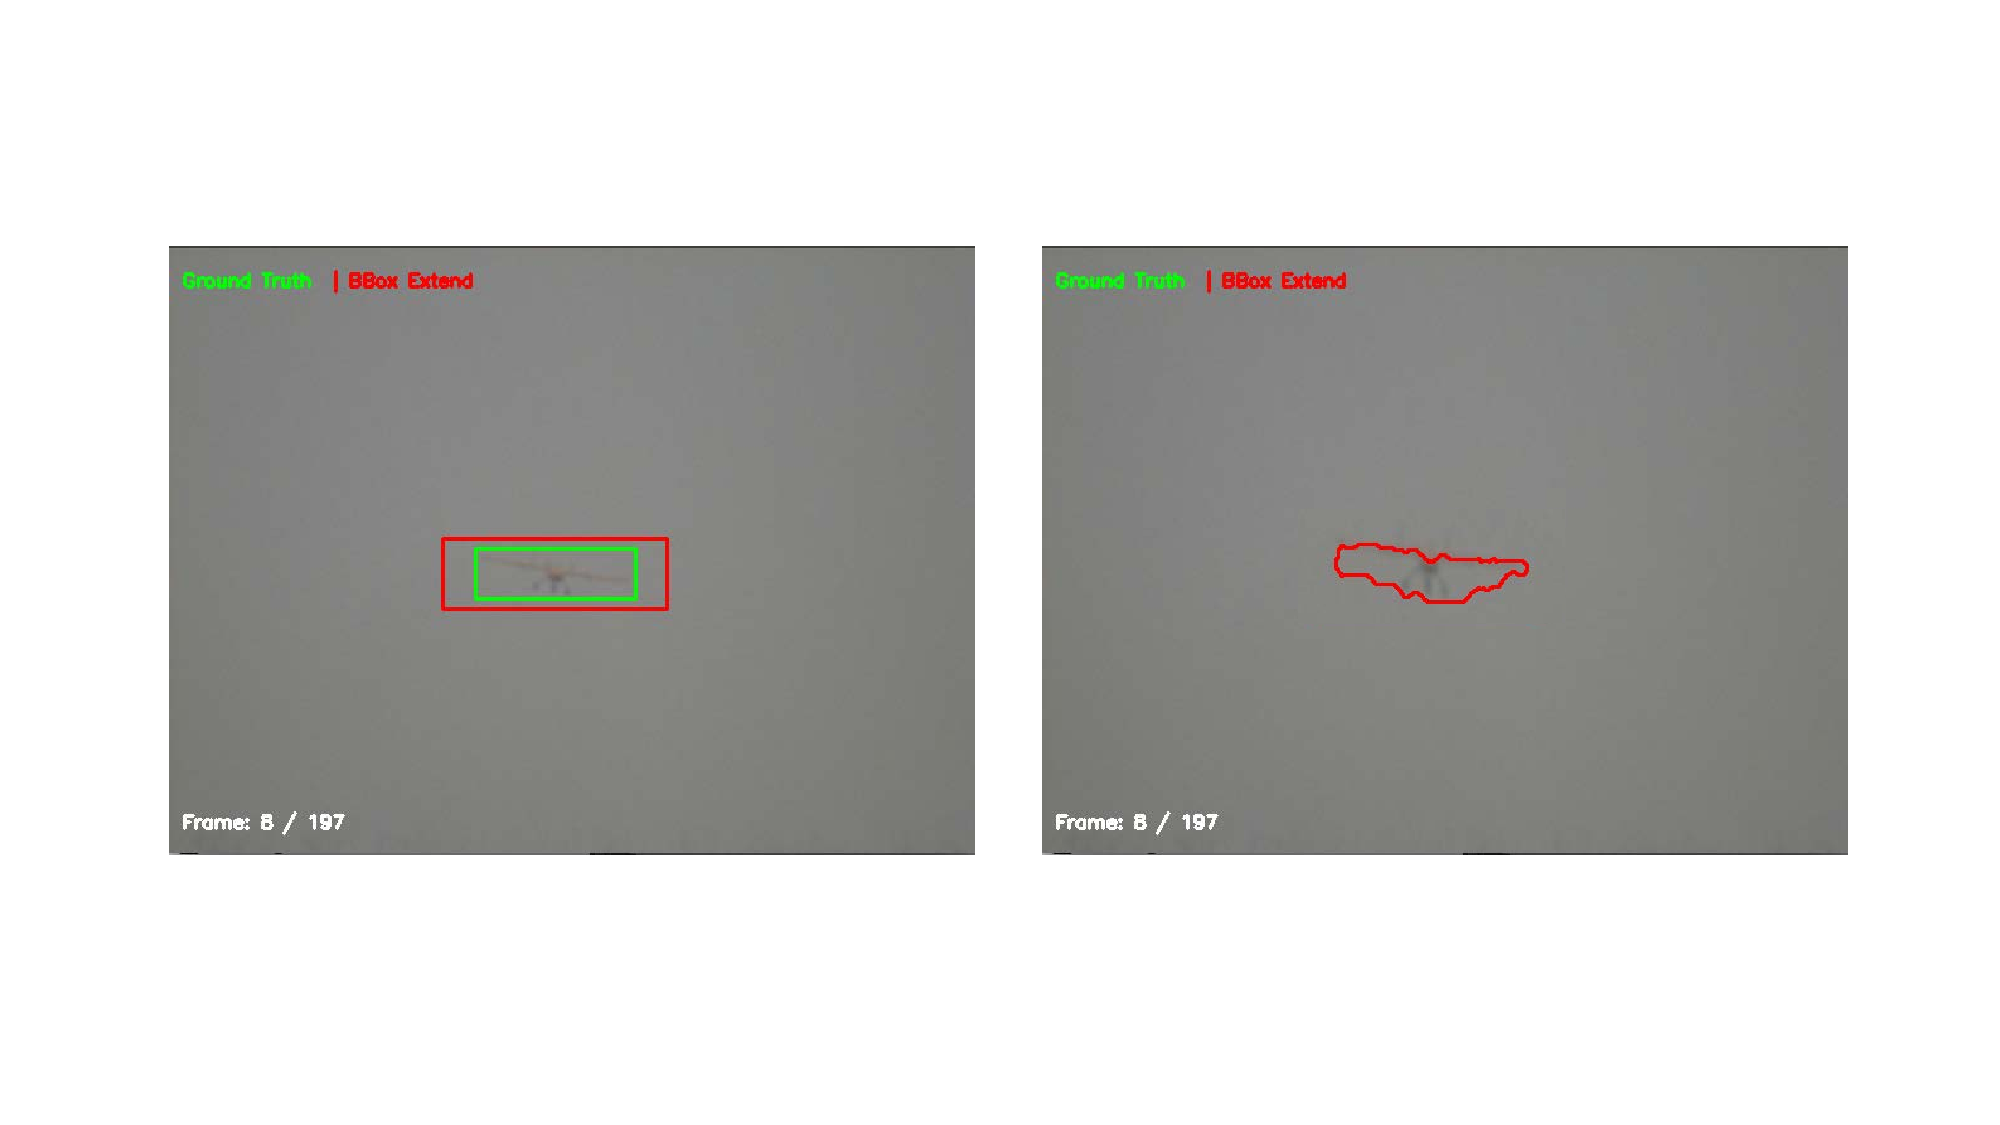
\includegraphics[width=0.8\textwidth]{Figs/chp04_07_active_contour_demo.pdf}
	\caption{Active Contour Algorithm}
	\label{fig:chp04_07_active_contour_demo}    
\end{figure}

%\subsection{PTU Attitude Compensation}




\section{Experiments and Discussion}
\subsection{UAV Platform}
In our on-board system we can see three components: The autopilot design allowed for the aircraft to perform simple commanded maneuver. The aircraft was flying at 60 m altitude at 25 m/s. This experimental test-bed is also a customized fixed wing aircraft as shown in Fig. \ref{fig:Kaitudozhe_VIGA}. It is a gasoline-powered radio-controlled model aircraft approximately 2.3 m in length and capable of lifting approximately 5 kg of payload. Table \ref{tab:platform_specifications} lists the other technical specifications.


\begin{figure}[!tb]
	\centering
	\subfigure[]
	{
			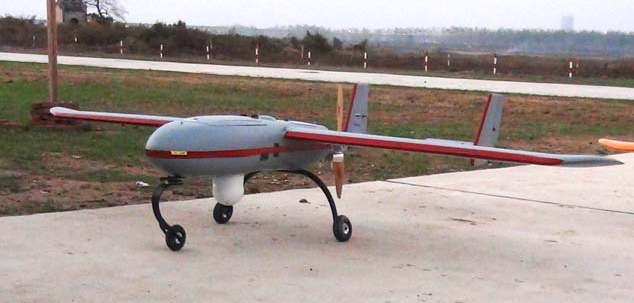
\includegraphics[height=3cm]{Figs/Kaituozhe_Our.pdf}
			\label{fig:Kaitudozhe_VIGA}
	}	
	\subfigure[]
	{
		\label{fig:iFly_F1A}
		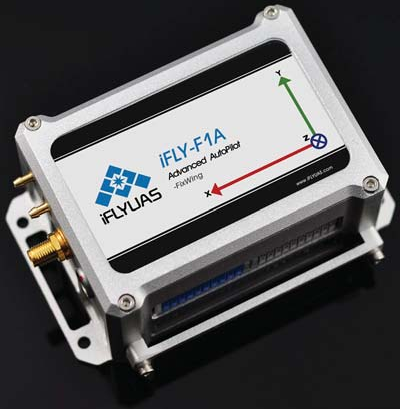
\includegraphics[height=3cm]{Figs/iFly_F1A.pdf}
	}
	\subfigure[]
	{
		\label{fig:iFly_G2}
		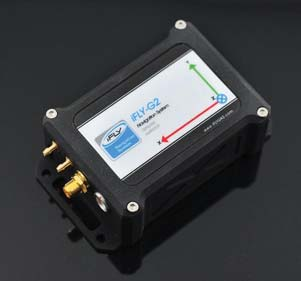
\includegraphics[height=3cm]{Figs/iFly_G2.pdf}
	}	
	\caption{(a) The Pioneer fixed-wing platform (b) iFLY-F1A Module   (c) iFLY-G2 Module}
\end{figure}



\begin{table}
	\caption{The Technical Specifications of Pioneer}
	\label{tab:platform_specifications}
	\begin{center}
		\renewcommand{\arraystretch}{1.1}
		\begin{tabular}{lll}
			\hline
			\textbf {Items}  & \textbf{Description} \\
			\hline
			Vehicle mass & 9000 g \\
			Maximum Payload mass & 5000 g \\
			Diameter & 2900 mm \\
			Flight duration & up to 180 minutes \\
			Cruising speed & 30.0 m/s \\
			\hline
		\end{tabular}
	\end{center}
\end{table}


The autopilot module is iFLY-F1A (Fig. \ref{fig:iFly_F1A}. It consists of the F1A autopilot system, a ground control station, a redundant power management module and an engine RPM monitoring module. We further make use of the iFLY-G2 (Fig. \ref{fig:iFly_G2} navigation autopilot module \cite{IFLY}, which is a small six-DOF (degree of freedom) navigation system. The G2 module includes a triaxial gyro, triaxial accelerometer, triaxial magnetometer, GNSS module, barometric altimeter, airspeed gauge and thermometer. It supports real-time 3D information including attitude angle, angular rate, position, speed, acceleration, true air speed, calibrated air speed. F1A is connected with G2 through RS-232 serial port.



Communication is curcial in the landing guidance framework, because the relative localization is broadcast through the radio. The guidance data are sent using an advanced radio modem that transmits and receives on the $900\ Mhz$ band. The XTend RF Modems support up to $22\ km$ outdoor communication with the interface data rates from $10\ bps$ to $230,00\ bps$, which is sufficient to transfer GNSS data and predicted position from ground station to on-board navigation modem.

 



\subsection{SRC-TLD Experiments}
To compare with the standard TLD method, the stability of Semi-random Code method was estimated for each frame by means of running 1000 Monte-Carlo experiments in one landing image sequence. Tabel \ref{lab:TLD_params} lists the parameters for TLD and SRC-TLD and the result is shown as \ref{fig:chp04_24_random_semi_random_monte_carlo}. The line shows the center location error for each algorithm, and the continuous shaded area is the error region, which explicate that the SRC has better stability and the accuracy of center location is improved. 

\begin{table}[!ht]
	\centering
	\caption{Parameters for TLD and SRC-TLD}
	\label{lab:TLD_params}
	\begin{tabular}{cc}
		\hline
		& \textbf{Parameters} \\ \hline
		Min/Max Scale & 10 \\
		Features Number & 10 \\
		Trees Number & 15 \\
		Learning Ratio & 0.8 \\ \hline
	\end{tabular}
\end{table}

\begin{figure}[!th]
	\centering
	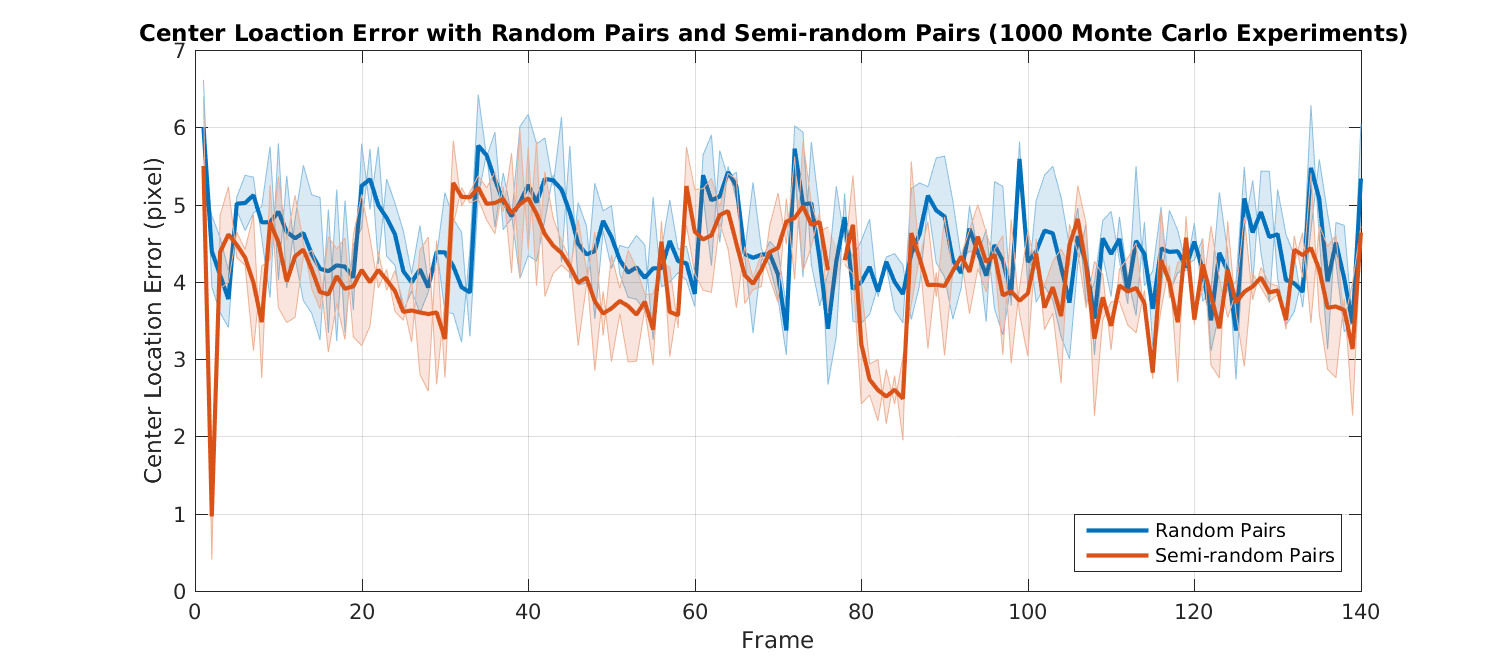
\includegraphics[width=0.8\textwidth]{Figs/chp04_24_random_semi_random_monte_carlo.pdf}
	\caption{Comparision between random and semi-random coding}
	\label{fig:chp04_24_random_semi_random_monte_carlo}    
\end{figure}

Also, we compared SRC-TLD with Meanshift, AdaBoost and standard TLD methods under different situations. The results was shown in Fig.\ref{lab:TLD_with_others}. The center location error of our methods are all within 7 pixel accuracy, which is the best compare with the other real-time tracking algorithms.
\begin{table*}[]
	\centering
	\caption{SRC-TLD Method Comparing with Other Tracking Algorithms}
	\label{lab:TLD_with_others} 
		\begin{tabular}{ccccccc}
			\hline
			\multicolumn{1}{l}{\multirow{2}{*}{}}                               & \multirow{2}{*}{Sequence} & \multirow{2}{*}{Frames} & AdaBoost     & Meanshift     & TLD          & \begin{tabular}[c]{@{}c@{}}TLD with \\ Semi-Random Pair\end{tabular} \\ \cline{4-7} 
			\multicolumn{1}{l}{}                                                &                           &                         & \multicolumn{4}{c}{Center Location Error(pixel) / Speed(fps)}                                                     \\ \hline
			\multirow{4}{*}{\begin{tabular}[c]{@{}c@{}}Small-sized\\ UAV\end{tabular}} & 1                         & 355                     & 6.31 / 9.51  & 14.39 / 15.35 & \textbf{6.14} / 21.13 & 6.20 / \textbf{21.22}                                                         \\
			& 2                         & 384                     & 7.47 / 10.81 & 14.25 / 15.11 & 6.37 / 20.91 & \textbf{6.31} / \textbf{21.19}                                                         \\
			& 3                         & 340                     & 6.61 / 10.14 & 13.48 / 15.33 & 5.62 / \textbf{21.10} & \textbf{5.23} / 20.60                                                         \\
			& 4                         & 338                     & 7.77 / 10.12 & 13.85 / 14.71 & 5.72 / \textbf{20.92} & \textbf{5.88} / 20.82                                                         \\ \hline
			\multirow{3}{*}{\begin{tabular}[c]{@{}c@{}}Middle-sized\\ UAV\end{tabular}} & 1                         & 137                     & 8.01 / 8.33  & 11.41 / 13.33 & 7.85 / \textbf{17.00} & \textbf{5.99} / 16.10                                                         \\
			& 2                         & 159                     & 9.65 / 8.59  & 13.10 / 13.67 & 6.95 / 16.96 & \textbf{5.12} / \textbf{16.97}                                                         \\
			& 3                         & 181                     & 8.33 / 8.01  & 11.13 / 13.03 & 6.93 / 17.37 & \textbf{5.39} / \textbf{17.77}                                                         \\ \hline
		\end{tabular}%
 
\end{table*}

 
 
%TODO:
%Effect of Ship Motion on the Automatic Landing Performance of a UAV - Navy Safety Boundaries

\subsection{Field Experiments}
\subsubsection{Scenarios}

The landing procedure were divided into four sections: (1) The UAV takeoff from the runway. (2) Cruise near the landing area in a large range to test the control system. (c) Cruise near the landing area in a small range and after the UAV is locked by visual system and received the visual references, the UAV control system was using vision-based localization data and the GPS data was only recorded as the benchmark. (d) Safely landing back to the runway.

 

%%% Selected Sentences



\subsubsection{Real-flight Experiments}
Based on the results of simulation,  seven sets of experimental results are conduced to establish the feasibility of the proposed approach. In realistic application, it is very critical requirements that the lateral deviation error from the middle line of the runway and the lateral acceleration of the vehicle should be perfectly eliminated to minimize the damage of the vehicle.
\begin{figure*}[!th]
	\centering
	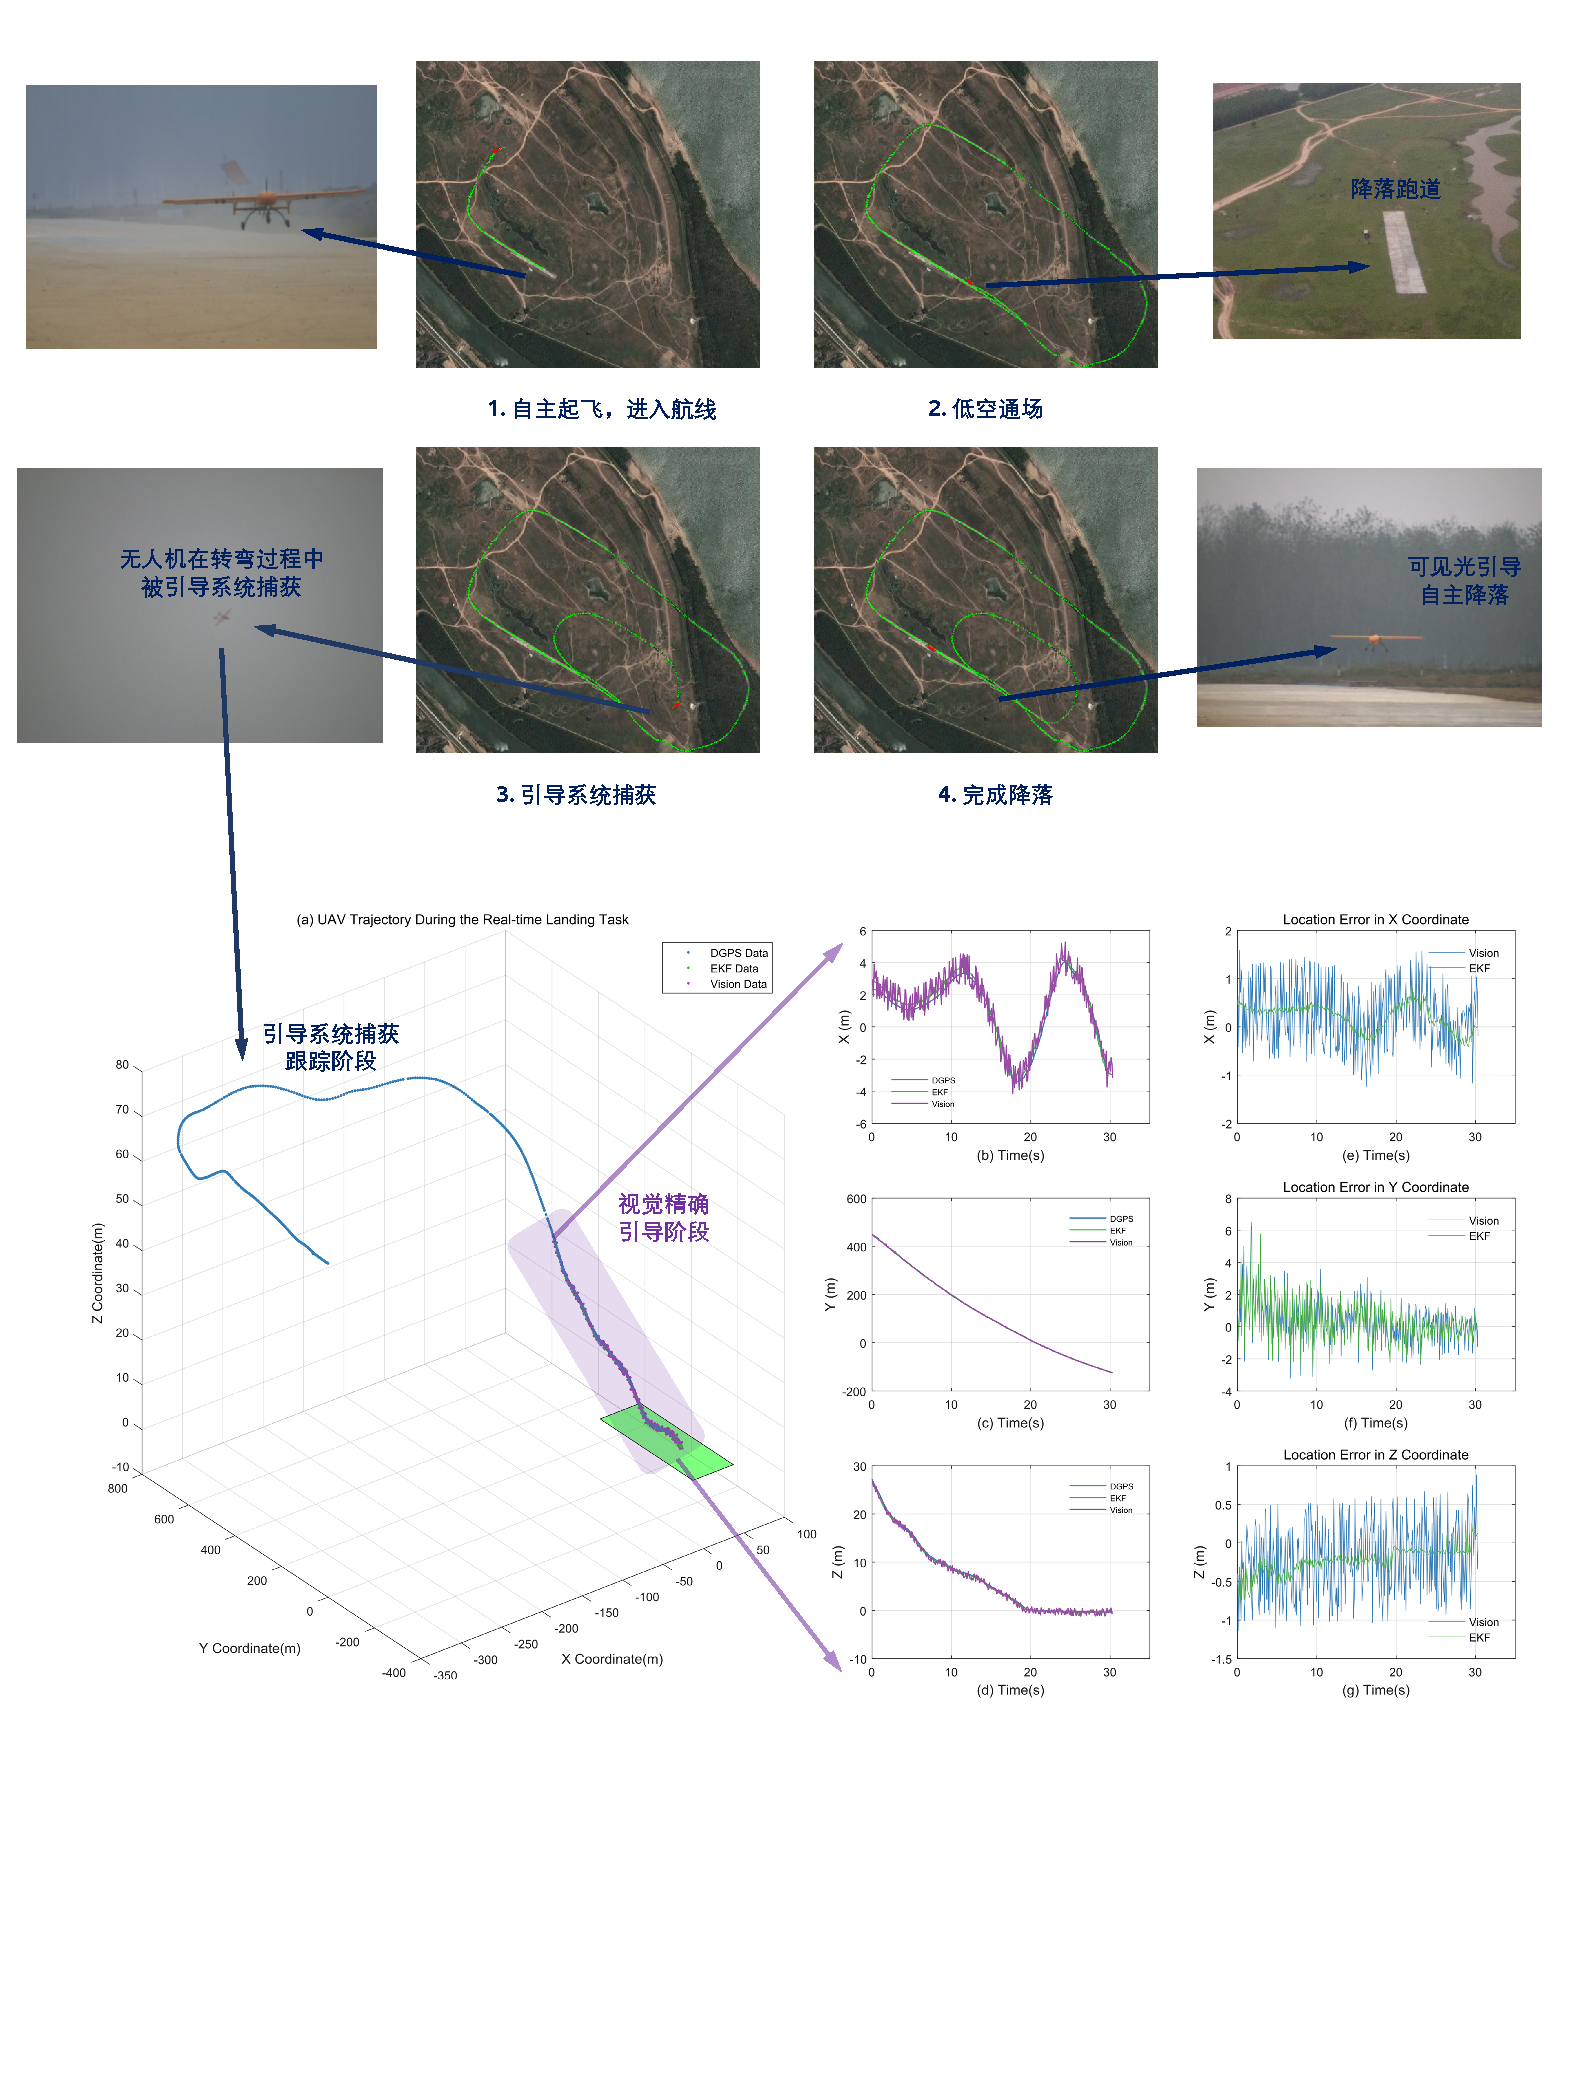
\includegraphics[width=0.8\textwidth]{Figs/chp08_23_ground_landing.pdf}	
	\caption{Ground Landing Processure}
	\label{fig:chp08_23_ground_landing}
\end{figure*}


\begin{table*}[!th]
	\centering
	\caption{Eight Experiment Results in Different Weather Condition}
	\label{lab:eight_ground_landing}
	\begin{tabular}{cccccc}
		\hline
		\multicolumn{1}{l}{\textbf{No.}} & \multicolumn{1}{l}{\textbf{Weather Condition}} & \multicolumn{1}{l}{\textbf{Detection Distance}} & \multicolumn{1}{l}{\textbf{RMSE $\mathbf{i}^{O,c}$(m)}} & \multicolumn{1}{l}{\textbf{RMSE $\mathbf{j}^{O,c}$(m)}} & \multicolumn{1}{l}{\textbf{RMSE $\mathbf{k}^{O,c}$(m)}} \\ \hline
		\textbf{1} & Clear & 848.735 & \underline{0.325} & \underline{1.451} & 0.280 \\
		\textbf{2} & Clear & \textbf{892.134} & 0.239 & 1.281 & \textbf{0.212} \\
		\textbf{3} & Clear & 872.311 & 0.373 & 1.319 & 0.282 \\
		\textbf{4} & Clear & \underline{847.373} & 0.259 & 1.401 & 0.233 \\
		\textbf{5} & Clear & 857.117 & \textbf{0.242} & \textbf{1.241} & \underline{0.301} \\ \hline
		\textbf{6} & Overcast & \underline{491.193} & \underline{0.491} & 1.676 & \underline{0.599} \\
		\textbf{7} & Overcast & 503.175 & 0.483 & \textbf{1.345} & \textbf{0.576} \\
		\textbf{8} & Overcast & \textbf{534.238} & \textbf{0.470} & \underline{1.772} & 0.581 \\ \hline
	\end{tabular}
\end{table*}


As the theoretical and simulation result discussed, the localization errors in each axis are large when the UAV is far way from the ground visual system. To illustrate the result more clearly, we compared the localization results with DGPS at separated intervals which is shown in Tabel. \ref{lab:ground_landing}.

\begin{table*}[!th]
	\centering
	\caption{Guidance Error in Each Axes at Separated Interval}
	\label{lab:ground_landing}
	\begin{tabular}{cccc|cccc}
		\hline
		\textbf{Interval(m)} & \textbf{$\mathbf{i}^{O,c}$(m)} & \textbf{$\mathbf{j}^{O,c}$(m)} & \textbf{$\mathbf{k}^{O,c}$(m)} & \textbf{Interval(m)} & \textbf{$\mathbf{i}^{O,c}$(m)} & \textbf{$\mathbf{j}^{O,c}$(m)} & \textbf{$\mathbf{k}^{O,c}$(m)} \\ \hline
		\textbf{600$\sim$580} & 0.332 & 1.856 & 0.431 & \textbf{300$\sim$280} & 0.128 & 1.426 & 0.171 \\
		\textbf{580$\sim$560} & 0.311 & 1.434 & 0.371 & \textbf{280$\sim$260} & 0.123 & 1.313 & 0.159 \\
		\textbf{560$\sim$540} & 0.208 & 1.542 & 0.300 & \textbf{260$\sim$240} & 0.104 & 1.104 & 0.114 \\
		\textbf{540$\sim$520} & 0.182 & 1.569 & 0.276 & \textbf{240$\sim$220} & 0.086 & 0.612 & 0.129 \\
		\textbf{520$\sim$500} & 0.217 & 1.863 & 0.180 & \textbf{220$\sim$200} & 0.099 & 0.882 & 0.131 \\
		\textbf{500$\sim$480} & 0.209 & 1.049 & 0.216 & \textbf{200$\sim$180} & 0.162 & 0.933 & 0.157 \\
		\textbf{480$\sim$460} & 0.185 & 1.478 & 0.253 & \textbf{180$\sim$160} & 0.154 & 0.730 & 0.136 \\
		\textbf{460$\sim$440} & 0.198 & 1.245 & 0.243 & \textbf{160$\sim$140} & 0.134 & 0.922 & 0.201 \\
		\textbf{440$\sim$420} & 0.171 & 1.412 & 0.151 & \textbf{140$\sim$120} & 0.143 & 0.696 & 0.125 \\
		\textbf{420$\sim$400} & 0.186 & 1.674 & 0.119 & \textbf{120$\sim$100} & 0.172 & 0.900 & 0.118 \\
		\textbf{400$\sim$380} & 0.159 & 1.679 & 0.145 & \textbf{100$\sim$80} & 0.139 & 0.668 & 0.079 \\
		\textbf{380$\sim$360} & 0.153 & 1.527 & 0.197 & \textbf{80$\sim$60} & 0.170 & 0.696 & 0.067 \\
		\textbf{360$\sim$340} & 0.171 & 1.292 & 0.138 & \textbf{60$\sim$40} & 0.105 & 0.460 & 0.055 \\
		\textbf{340$\sim$320} & 0.164 & 1.360 & 0.217 & \textbf{40$\sim$20} & 0.126 & 0.276 & 0.082 \\
		\textbf{320$\sim$300} & 0.156 & 1.420 & 0.204 & \textbf{20$\sim$00} & 0.070 & 0.261 & 0.095 \\ \hline
	\end{tabular}
\end{table*}



\begin{figure*}[!t]
	\centering
	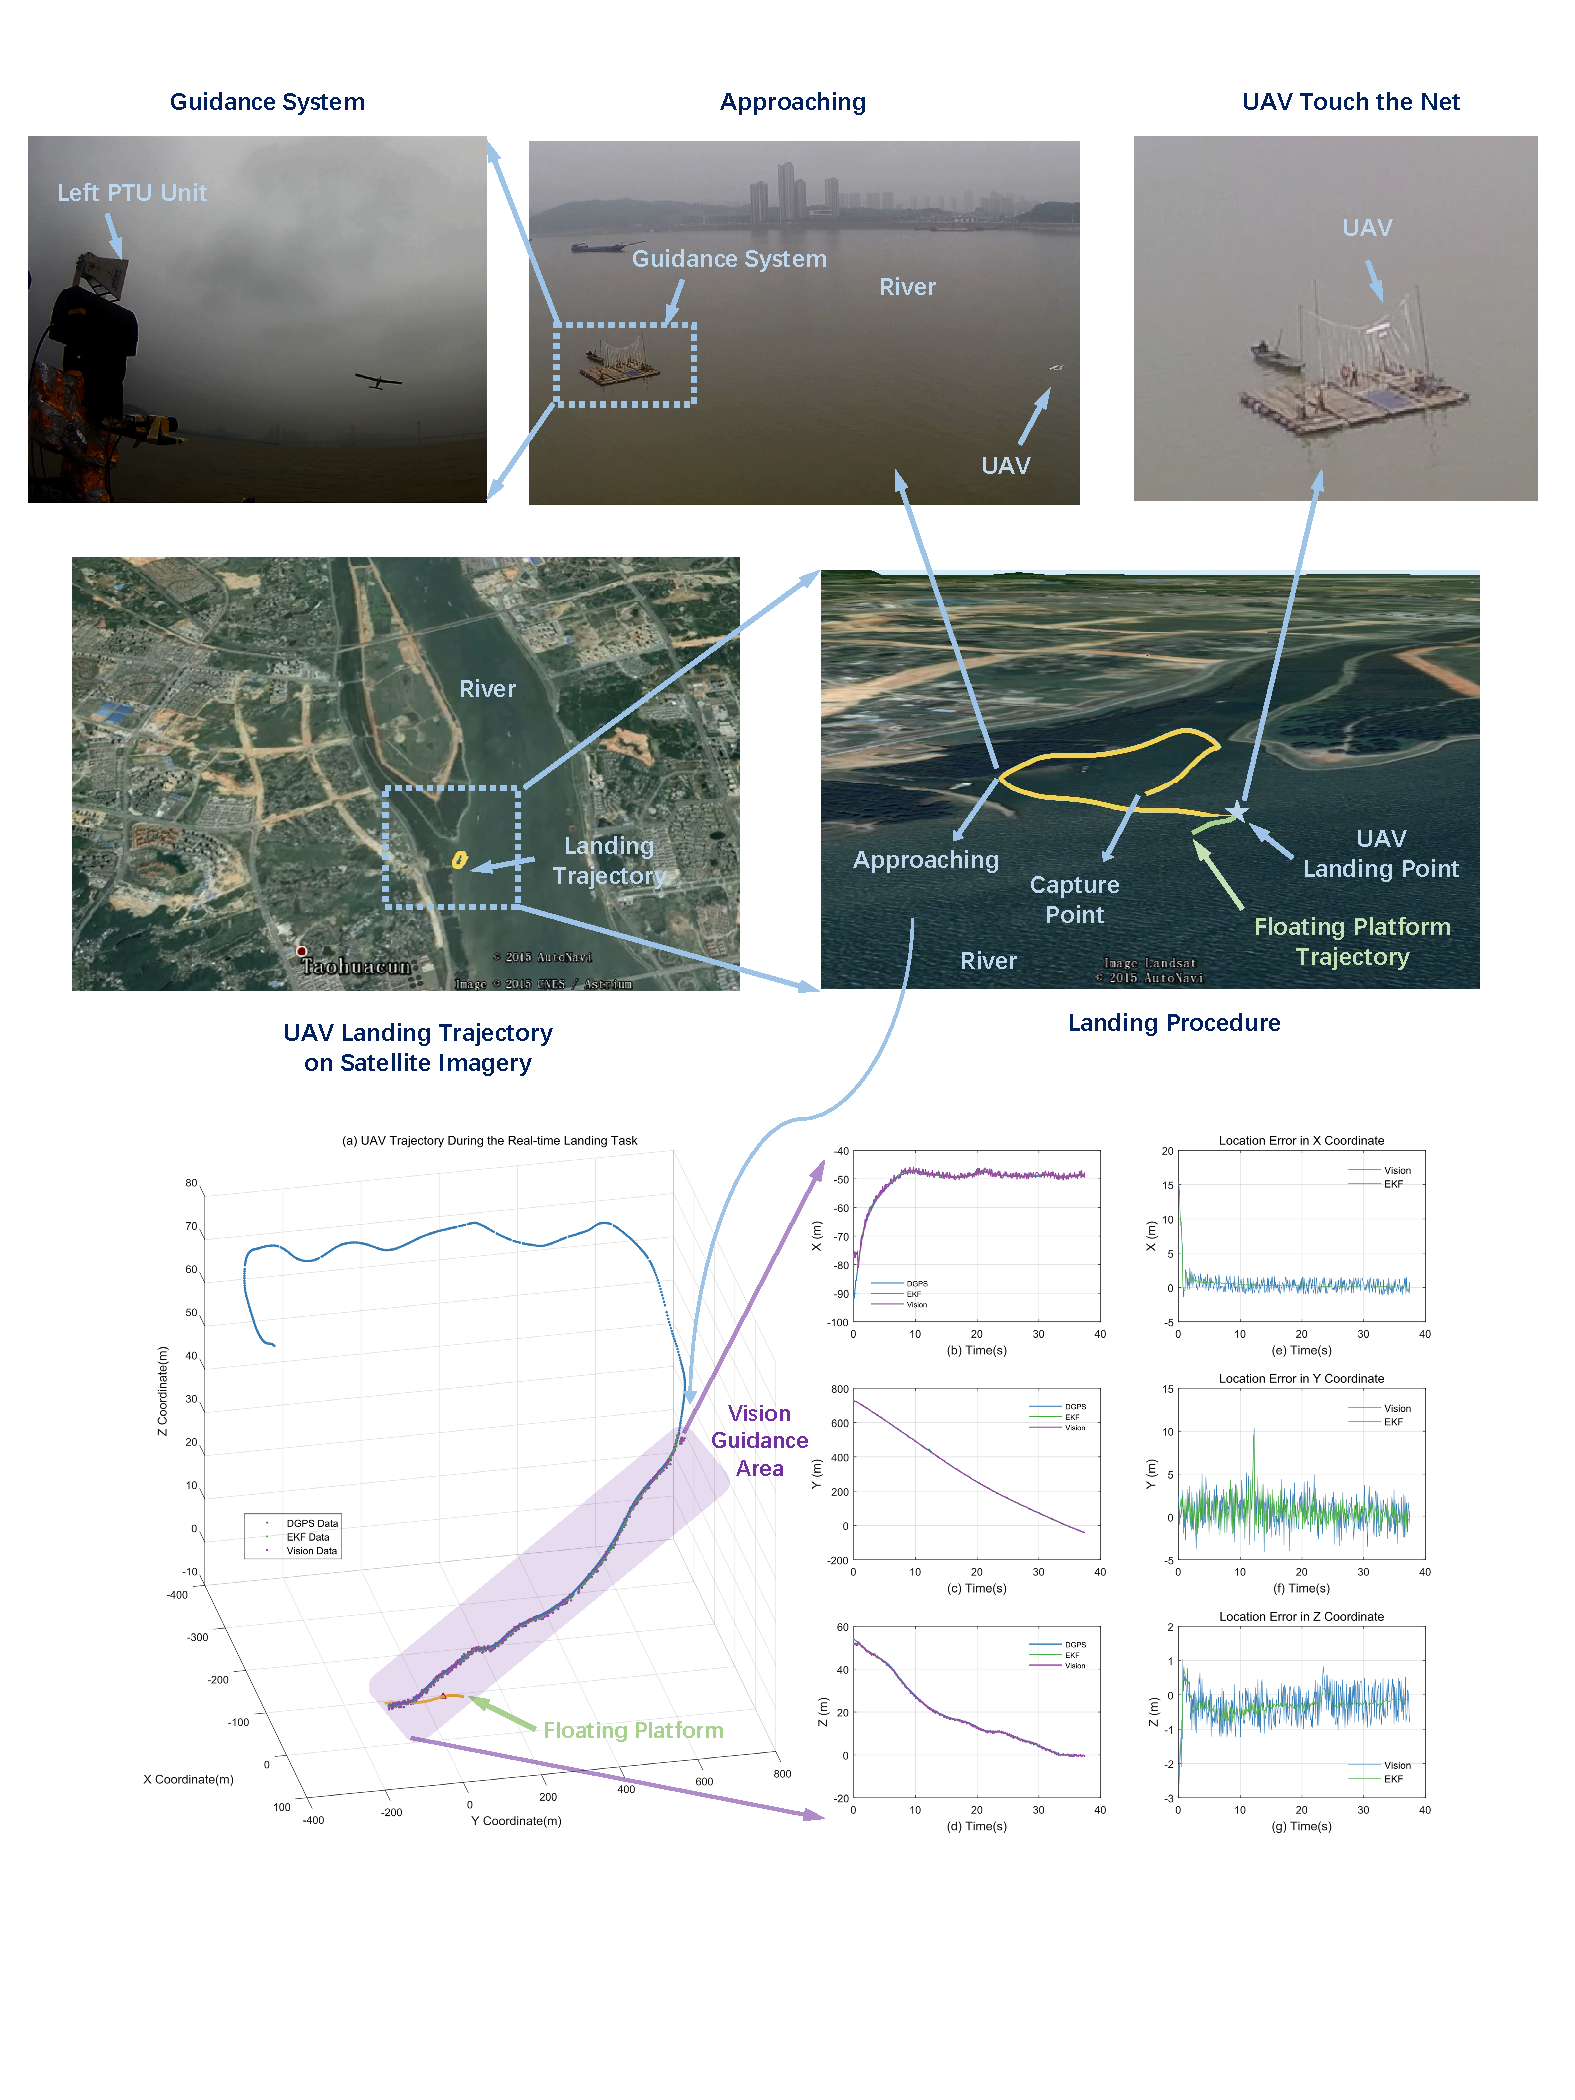
\includegraphics[width=0.8\textwidth]{Figs/chp08_21_river_landing.pdf}	
	\caption{Surface Landing Processure}
	\label{fig:chp08_21_river_landing}
\end{figure*}


\begin{figure*}[!ht]
	\centering
	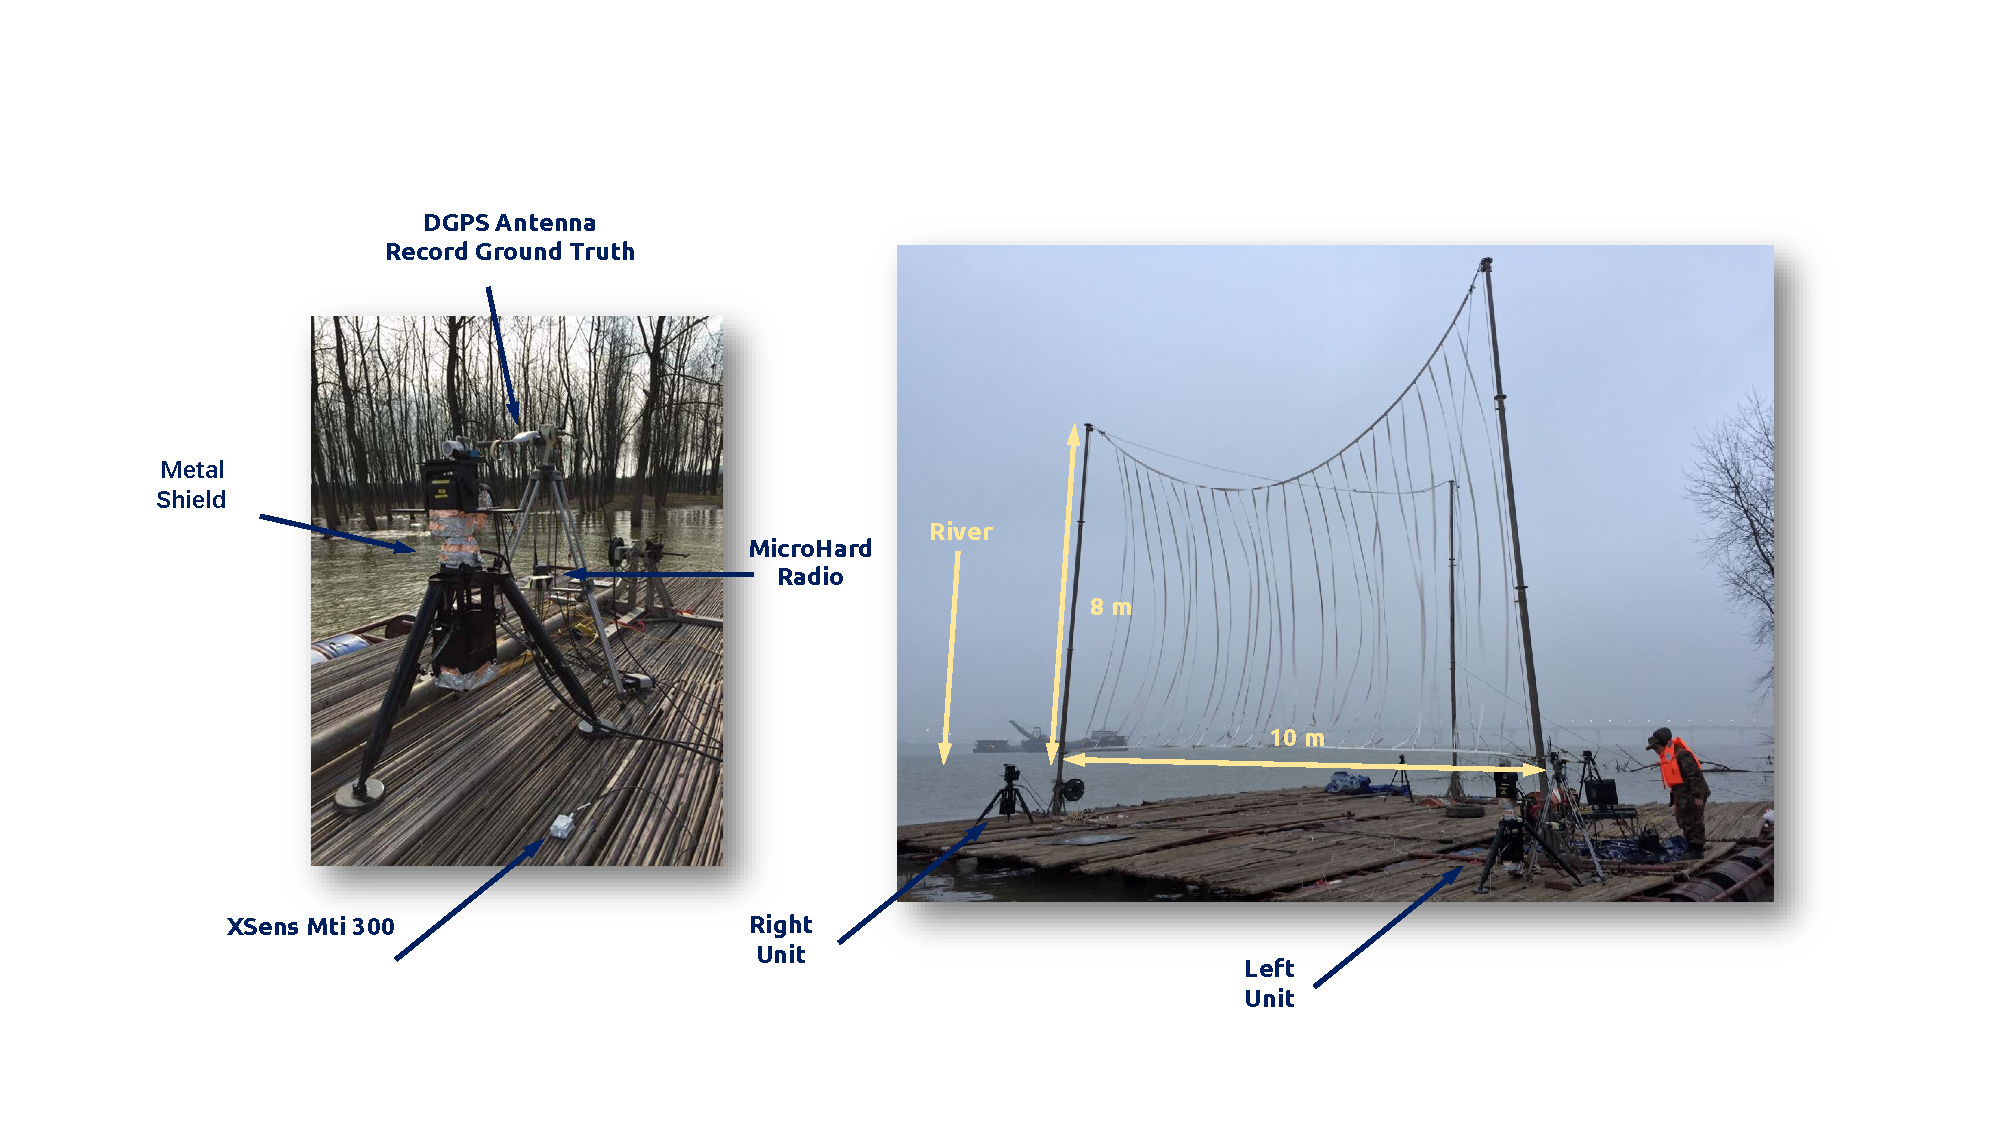
\includegraphics[width=0.8\textwidth]{Figs/chp08_16_ship_ptus.pdf}	
	\caption{Guidance Configuration on Floating Platform}
	\label{fig:chp08_16_ship_ptus}
\end{figure*}



\begin{table*}[!th]
	\centering
	\caption{Three Surface Landing Experiments Results}
	\label{lab:three_ship_landing}
	\begin{tabular}{cccccc}
		\hline
		\multicolumn{1}{l}{\textbf{No.}} & \multicolumn{1}{l}{\textbf{Weather Condition}} & \multicolumn{1}{l}{\textbf{Detection Distance}} & \multicolumn{1}{l}{\textbf{RMSE $\mathbf{i}^{O,c}$(m)}} & \multicolumn{1}{l}{\textbf{RMSE $\mathbf{j}^{O,c}$(m)}} & \multicolumn{1}{l}{\textbf{RMSE $\mathbf{k}^{O,c}$(m)}} \\ \hline
		\textbf{1} & Clear & 628.735 & 0.514 & 1.721 & 0.371 \\
		\textbf{2} & Clear & \textbf{632.134} & 0.547 & 1.363 & 0.342 \\
		\textbf{3} & Clear & \underline{622.311} & 0.583 & 1.571 & 0.389 \\ \hline
	\end{tabular}
\end{table*}

Our vision systems uses customized vision algorithms and off-the-shelf hardware to perform in real-time. Actual flight test results on our UAV testbed show our vision-based state estimates are accurate to within 5 cm in each axis of translation and 5 degrees in each axis of rotation.

\subsection{Conclusion}
This paper presents a complete framework of the ground-based stereo localization  problem and shows a real practical use case where the approach
presented could be used to guidance the UAV landing autonomously and safely in GNSS-denied scenario. Additional future work will focus on estimate errors over time and investigate methods to improve inevitable error propagation through the inclusion of additional sensors, such as GNSS sensor and on-board IMUs.



%% For tables use
%\begin{table*}
%% table caption is above the table
%\caption{Please write your table caption here}
%\label{tab:1}       % Give a unique label
%% For LaTeX tables use
%\begin{tabular}{lll}
%\hline\noalign{\smallskip}
%first & second & third  \\
%\noalign{\smallskip}\hline\noalign{\smallskip}
%number & number & number \\
%number & number & number \\
%\noalign{\smallskip}\hline
%\end{tabular}
%\end{table*}


%\begin{acknowledgements}
%If you'd like to thank anyone, place your comments here
%and remove the percent signs.
%\end{acknowledgements}

% BibTeX users please use one of
%\bibliographystyle{spbasic}      % basic style, author-year citations
%\bibliographystyle{spmpsci}      % mathematics and physical sciences
%\bibliographystyle{spphys}       % APS-like style for physics
%\bibliography{template}   % name your BibTeX data base

% Non-BibTeX users please use
%\begin{thebibliography}{}
%
% and use \bibitem to create references. Consult the Instructions
% for authors for reference list style.
%
%\bibitem{RefJ}
% Format for Journal Reference
%Author, Article title, Journal, Volume, page numbers (year)
% Format for books
%\bibitem{RefB}
%Author, Book title, page numbers. Publisher, place (year)
% etc
%\end{thebibliography}

% BibTeX users please use one of
%\bibliographystyle{spbasic}      % basic style, author-year citations
%\bibliographystyle{spmpsci}      % mathematics and physical sciences
%\bibliographystyle{usrt} % by Kong
%\bibliographystyle{spphys}       % APS-like style for physics

%\bibliography{template}   % name your BibTeX data base
%\printbibliography
\bibliographystyle{IEEEtran}
\bibliography{template}

\end{document}
% end of file template.tex

